%!TEX program = xelatex
% 完整编译: xelatex -> bibtex -> xelatex -> xelatex
\documentclass[lang=cn,11pt,a4paper]{paper}

\title{基于地点的补贴式租赁住房的挤出效应:来自LIHTC项目的新证据}
\author{Michael D. Eriksen\thanks{\href{http://www.eriksen.myweb.uga.edu}{迈克尔·D·埃里克森},电话:+1 706 542 9774,传真:+1 706 542 4295,电子邮件:\email{eriksen@terry.uga.edu}。佐治亚大学特里商学院房地产系,美国乔治亚州雅典城,GA 30602。} \and Stuart S. Rosenthal\thanks{\href{http://www.faculty.maxwell.syr.edu/rosenthal}{斯图亚特·S·罗森塔尔},通讯作者,电话:+1 315 443 3809,传真:+1 315 443 1081,电子邮件:\email{ssrosent@maxwell.syr.edu}。锡拉丘兹大学经济系和政策研究中心,美国纽约锡拉丘兹,13244-1020。}\; \thanks{\href{https://www.sciencedirect.com/science/article/pii/S0047272710000885}{\faLink\;英文原文链接},\href{https://sci-hub.tw/10.1016/j.jpubeco.2010.07.002}{\faFilePdf[regular]\;PDF 下载}。作者非常感谢John D.,Catherine T. MacArthur 基金会,Ford 基金会以及住房和城市发展部为该项目提供的资金。本文从许多人的有价值的评论中受益。我们感谢两位匿名评审人,Dennis Epple(编辑),Denise DiPasquale,Gary Engelhardt,Jeffrey Kubik,Edgar Olsen,Erika Poethig,Steve Ross,Michael Stegman,Bruce Weinberg,Johnny Yinger,以及2007年1月AREUEA会议的参与者和俄亥俄州立大学提供的有益意见。当然,文责自负。}}
\translator{翻译者:\href{https://tomben.me}{任\ 涛}}

\date{\zhtoday}

\begin{document}

\maketitle

\begin{abstract}
  \hspace{2\ccwd}自1987年成立以来,低收入住房税收减免项目(the Low Income Housing Tax Credit, LIHTC)已迅速发展成为美国有史以来规模最大的低收入住房补贴建设来源,占最近所有多户家庭出租房屋的三分之一。本文研究了这种日益重要的中低收入住房来源的挤出效应。为此,我们从MSA,县和10英里半径圆这三个不同的地理层面分析了LIHTC建设的影响。这使我们能够采用越来越广泛的地域固定因子,以识别未被观察到的因素。此外,政治变量也被用作进一步促进识别的工具。
  
  \!在我们所有的模型中,IV估计产生的挤出效应要比OLS大得多,这证实了LIHTC开发对新建筑成熟区域的内生吸引力。我们最可靠的IV估算表明,几乎100\%的LIHTC建设被新建的无补贴租赁单位的数量的减少所抵消,尽管这一点估计值附近的置信区间不能让我们作出关键的评价。其他估算表明,LIHTC的发展对自住房建设的影响要小得多,但这些估算并不非常精确。总体而言,尽管LIHTC的发展可能会很好地影响低收入公寓的位置,但我们的估计表明,该计划对新开发的出租房屋数量的影响似乎很小。

  \keywords{挤出效应,保障性住房,LIHTC}
\end{abstract}
\vspace{10pt}

\begin{tcolorbox}[
	colback=yellow!10!white,
  colframe=red!30!black,
  fontupper = \itshape,
]
“I rise today to introduce the Affordable Housing Tax Credit Enhancement Act of 2005. … the bill would double the current LIHTC [annual allocations], which would yield twice the number of affordable units annually. … Today, the LIHTC program is widely regarded as the nation's most successful housing production program resulting in the construction and rehabilitation of more than 1.3 million housing units for lower income households. …”
\vspace{5pt}

\textbf{Statements Submitted to Congressional Record: May 26, 2005 By Rep. William Jefferson (D-LA)}

\tcblower

“我今天起草来介绍《2005年经济适用房税收抵免补充法案》。……该法案将使目前的LIHTC(年度拨款)翻一番,这将使每年的经济适用房数量增加一倍… 今天,LIHTC计划被公认为是美国最成功的住房保障计划,它为低收入家庭建造和翻新了130万套住房……”
\vspace{5pt}

\textbf{众议员William Jefferson(D-LA)在2005年5月26日提交国会的发言录音。}

\end{tcolorbox}
\vspace{10pt}

\section{引言}

提供给低收入群体的住房援助方式仍然有很多甚至是激烈的争论:政府应该通过需求端优惠政策(例如第8节优惠券),还是通过类似公共住房或住房税收抵免政策(LIHTC)补贴供给端建设成本?在此背景下,本文考察了快速增长的LIHTC计划,并强调了LIHTC建设在多大程度上挤压了无补贴租赁房屋的开发,一些进一步的背景将有助于正确看待LIHTC项目。

20世纪30年代末至80年代中期,联邦政府通过“传统”公共住房计划建造了超过一百万套住房。重要的是,这些项目通常将入住群体限制在接近或低于贫困水平的家庭 \citep{Olsen2003365}\,\footnote{\cite{Olsen2003365}指出,至少有29种不同的公共住房计划。 这些项目中的家庭通常将其总收入的30\%用于房租。}。到20世纪80年代,至少在两个方面,人们的担忧开始削弱政府对公共住房进一步扩大的支持。 首先是政府建设,拥有和运营公共住房项目。 关于某些活动是否最好留给私营部门存在一些基本问题。第二个是公共住房项目造成了密集的贫困集聚,加剧了人们对犯罪,邻里关系恶化,以及对儿童成长的不利影响的担忧,例如可参见 \cite{Currie200099,Jencks1990111}。出于这些原因,公共住房建设在20世纪80年代初就结束了,20世纪90年代开始拆除最差的一些项目\,\footnote{在某些情况下,例如根据HOPE VI项目,公共住房结构进行了改建,但在大多数情况下,通常是向住户发放住房券,并让他们自己去寻找住房 \citep{Jacob2004233}。}。

随着1986年的税收改革法案(TRA86),低收入住房税收抵免(LIHTC)项目应运而生,作为公共住房的替代方案,同时也抵消了改革对出租住房业主的其他税收优惠的减免\citep{USCongress1987}\,\footnote{根据美国税法第42条,LIHTC计划由国税局管理。}。LIHTC项目的前提与公共住房明显不同,它是基于政府和营利性开发商之间的合作关系。根据LIHTC的规定,私人开发商可以从非土地建设成本中获得高额补贴,如果收入低于住房和城市发展部(HUD)规定标准的租户保留的公寓份额增加,补贴的力度也会随着增加\,\footnote{联邦政府通过一项为期10年的年度不可退还的联邦所得税减免,一美元对一美元地降低私人开发商的联邦所得税责任,补贴私人开发商30\% - 91\%的非土地建设成本 \cite{Eriksen2009141}。由于补贴的力度随着分配给低收入居民的项目单元份额的增加而增加,大多数开发商的应对措施是让所有单元都住满符合收入标准的租户。不遵守LIHTC的操作规则将导致开发商丧失未来的税收减免,并偿还1/3拨款和利息。}。此外,开发商同意在至少15年内,将目标公寓的租金设定在规定的上限之下,之后才允许收取市场租金。考虑到这些规定,LIHTC在某些方面是一种有针对性的租金控制形式,入住资格规定限制了特定的人群。

LIHTC很快就超越了之前所有基于地点的补贴租赁项目,成为美国历史上规模最大的住房保障项目。在\tabref{tab1}中,值得注意的是,从1987年到2006年,LIHTC项目大约建设了160万套住房,约占近期所有多户型出租住房的三分之一,\figref{fig1}是过去60年公共住房的建设和LIHTC的发展,进一步说明了这一点\,\footnote{\figref{fig1}中的公共住房数据从住房和城市发展部的分析师处获得,并得到了John D., Catherine T. MacArthur和Abt Associates的帮助。这些数据在两个方面不同于 \url{http://www.huduser.org} 的公开数据:首先,我们的数据包含每个“项目”从1937年到2000年投入使用的年份,这能够代表每十年新建的公共住房。此外,我们的数据还包括20世纪90年代拆除的公共住房的信息。LIHTC的数据从 \url{http://www.lihtc.huduser.org} 获得。}。最近LIHTC繁荣的发展是显而易见的,同样明显的是,在\tabref{tab2}中,尽管LIHTC计划的成本相对于住房券计划来说似乎不算高,但LIHTC计划的绝对成本却很高。2006年,住房券项目耗资近210亿美元。相比之下,与LIHTC计划相关的联邦税收损失总计49亿美元。然而,由于从2001年开始分配的信贷增加了40\%,预计这一费用在未来几年将急剧增加\,\footnote{即使最近有关扩大LIHTC项目的议案尚未出台,这些增长也会发生。\cite{USCongress2005} 的一份报告,提供了有关各种形式的低收入者住房支助费用的详细资料。}。

\begin{table}[h]
\centering
\setlength{\tabcolsep}{12mm}
  \begin{threeparttable}
  \caption{国家LIHTC汇总统计\tnote{a}}\label{tab1}
    \begin{tabular}{ccc}
  \toprule
  & 年度拨款总额 (\$)\tnote{b}
  & 补贴单位数量\tnote{c} \\
  \midrule
  1987 & 980,533,493 & 34,491 \\
  1988 & 3,140,987,971 & 81,408 \\
  1989 & 4,387,952,511 & 126,200 \\
  1990 & 2,888,647,156 & 74,029 \\
  1991 & 5,207,469,242 & 111,970 \\
  1992 & 4,255,013,370 & 91,300 \\
  1993 & 5,205,992,598 & 103,756 \\
  1994 & 5,915,192,114 & 117,099 \\
  1995 & 4,892,206,044 & 86,343 \\
  1996 & 4,277,723,133 & 77,003 \\
  1997 & 4,225,625,522 & 70,453 \\
  1998 & 3,999,808,231 & 67,822 \\
  1999 & 3,983,473,499 & 62,240 \\
  2000 & 3,895,882,268 & 59,601 \\
  2001 & 4,624,992,306 & 67,261 \\
  2002 & 5,162,994,677 & 69,310 \\
  2003 & 5,507,541,467 & 73,877 \\
  2004 & 5,680,347,051 & 75,600 \\
  2005 & 5,556,042,690 & 70,630 \\
  2006 & 6,668,538,964 & 74,278 \\
  总计 & 90,456,964,308 & 1,594,671 \\
  \bottomrule
    \end{tabular}
  \begin{tablenotes}
    \footnotesize
    \item[a] 数据由国家住房当局全国委员会汇编。
    \item[b] 计算时假设通货膨胀率为3\%,并且在分配后的10年内将申请已分配的税收抵免。
    \item[c] 不包括未补贴的市场价格单位,有时包括在LIHTC补贴的房产中。
  \end{tablenotes}
\end{threeparttable}
\end{table}

\begin{figure}[h]
	\centering
	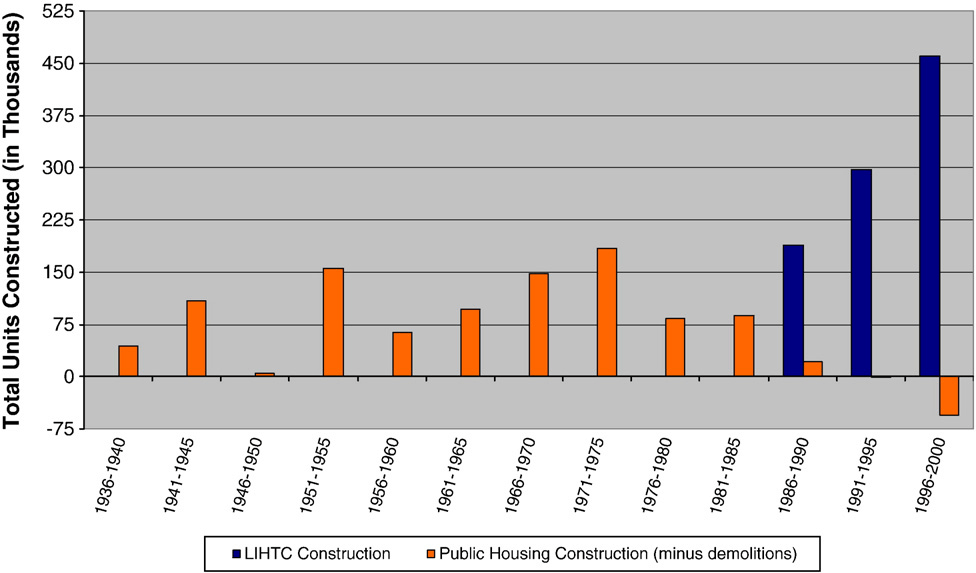
\includegraphics[width=16cm]{fig1.png}
	\caption{基于地点的住房补贴建造和拆除}\label{fig1}
\end{figure}

\renewcommand\arraystretch{0.9}
\begin{table}[h]
  \centering
  \setlength{\tabcolsep}{12mm}
    \begin{threeparttable}
    \caption{联邦政府低收入住房支出(2005-2006)(单位:百万美元)\!\!\tnote{a}}\label{tab2}
      \begin{tabular}{ccc}
        \toprule
        & 2005 & 2006 \\
        \midrule
        \textbf{国税局}\tnote{b} & & \\
        低收入住房税收抵免 & 4700 & 4900 \\
        优惠折旧免税额 & 3800 & 4200 \\
        国家发行的租赁住房免税融资 & 300 &
        300 \\[5pt]
        \textbf{住房和城市发展部}\tnote{c} & & \\
        住房选择券(HCV) & 20,064 & 20,917 \\
        公共住房 & 5017 & 5734 \\
        其他HUD项目 & 8734 & 4559 \\[5pt]
        \textbf{农业部}\tnote{c} & & \\
        农村住房管理 & 1369 & 1029 \\
        总计 & 43,984 & 41,639 \\
        \bottomrule
      \end{tabular}
    \begin{tablenotes}
      \footnotesize
      \item[a] LIHTC成本反映了与10年税收抵免分配相关的税收损失。鉴于自2001年以来LIHTC拨款的增加,这些费用预计将在未来几年大幅增加。随着越来越多的公共住房单元被拆除,未来几年公共住房运营成本可能会下降。
      \item[b] 根据 \cite{USCongress2005} 估算的税收支出。
      \item[c] 美国政府预算,\cite{Budget2006}。
    \end{tablenotes}
  \end{threeparttable}
  \end{table}

很明显,LIHTC是一个昂贵的项目。同样明显的是,LIHTC是一种有针对性的租金控制形式。但不太明显的是,LIHTC实际上针对的是中等收入的租户,而不是低收入租户。在考虑LIHTC计划的挤出效应时,这一点尤其重要,无论是在总体上还是在公共住房方面。尽管私营部门很少为接近或低于贫困线的家庭建造无补贴住房,但他们通常为中等收入群体建造出租住房。这表明,虽然建造公共住房只是间接地与未受资助的私人开发项目竞争,但LIHTC项目与未受资助的建筑项目直接竞争。因为挤出是在政府与私营部门争夺市场份额时出现的,所以以中等收入家庭为目标对象,增大了LIHTC项目取代无补贴开发的可能性。鉴于LIHTC计划的这一特点的重要性,我们在提出下列四条观点,证实LIHTC倾向于以收入远高于传统公共住房的家庭为目标。

首先是LIHTC补贴住房的租金上限定得相对较高。准确地说,租金上限设定为区域内家庭收入的中位数,即18\%(Area Median Household Income, AMI,例如MSA中位收入。),每年由住房和城市发展部(HUD)规定\,\footnote{之所以提出18\%的AMI收入门槛,是因为补贴单位的居住者的收入必须低于AMI的60\%,而向补贴单位的个人收取的租金不得超过该上限的30\%。}。尽管每个城市的租金上限各不相同,但它们与住房和城市发展部规定的公平市场租金相近 \citep{Cummings1999257},后者用于调节第8节凭证领取者支付的租金。这些租金通常在上年私人市场合同租金的40\%到50\%之间。对于许多低收入家庭来说,这种水平的租金是负担不起的。

第二点也是相关的一点,LIHTC补贴住房租户的收入限制也定在相对较高的水平。具体而言,住房和城市发展部将LIHTC补贴单位的收入资格定为最低收入水平的60\%。这一限额远远高于传统公共住房开发居住者的收入限额\,\footnote{例如,住房和城市发展部规定,2000年华盛顿的一个三口之家规定的LIHTC收入限额为43,500美元(大约相当于该规模家庭家庭收入中位数的60\%)。LIHTC项目业主在那一年可以向这样一个家庭收取的最高租金是每月1088美元。相比之下,2000年华盛顿的所有出租住房(未补贴加补贴住房)的租金中位数为每月840美元。参见住房和城市发展部网站:\url{http://www.huduser.org}。}。

第三点是关于LIHTC单位的建筑质量。针对较高收入租户应该促使开发商提供更高质量的住房(因为住房是一种普通的商品)。\cite{Eriksen2009141} 使用1999年至2005年期间加州LIHTC发展的详细数据,得出了与上述观点一致的结论\,\footnote{\cite{Eriksen2009141} 还强调,由于LIHTC补贴非土地建设成本,而不是土地本身,要素价格替代效应会进一步激励开发商提高建筑质量。}。\cite{Eriksen2009141} 发现,LIHTC项目的非土地建设成本的中位数为每平方英尺128美元,他进一步说明,这比加州同期无补贴租赁住房开发的非土地成本中位数高出21\%。

很明显,LIHTC的开发项目受到相对较高的租金上限、支配资格的高收入限制以及高质量的建筑的制约。综上所述,这些特征表明,LIHTC租户的收入可能比公共住房租户的收入要高得多。\cite{Wallace1995785} 发现,只有28\%的LIHTC居民的收入低于AMI的50\% (AMI是HUD用来定义非常低收入的家庭的基准),他认为,传统公共住房开发项目中,81\%的居民收入非常低。鉴于上述证据和方案特点,很明显,LIHTC的目标是中等收入家庭,而不是低收入家庭。因此,LIHTC也有可能与未受资助的开发项目直接竞争,这增加了LIHTC项目取代未受资助建设项目的可能性。

为了评估LIHTC发展的挤出效应,我们将1990年的普查区域数据与1990年至2000年间LIHTC发展的信息相结合。我们的基本策略是对20世纪90年代LIHTC发展中的私营部门住房建设进行面板回归,控制先前文献中阐述的住房开工的其他驱动因素 \cite{Mayer200085}。\cite{Murray1999107} 在分析美国住房总量的时间序列时,强调的另一种方法是评估补贴住房建设对住房总量的影响。我们在后文部分认为,我们对新发展的关注产生了密切相关的结果,这些结果在我们的数据具有很大的跨部门性质的情况下更加可靠。特别的,我们所有的模型都是以住房存量的滞后水平为条件的(以及其他的描述性控制变量),这使得我们的因变量反映了1990年至2000年期间住房存量的变化,而不考虑因变量是被指定为住房存量的变化还是2000年住房存量的水平\,\footnote{注意,以$y_t=b_0+b_1y_{t-1}+b_2x_t$为例,等式两边同时减去$y_{t-1}$,只影响滞后因变量,而系数$x$不变。此外,\cite{Murray1999107} 试图分析保障性住房建设对住房均衡存量的影响,\cite{Murray1983590} 则侧重于保障性住房开发对住房开工率的影响。}。两个相关的实证挑战仍然存在,它们在我们挤出效应的分析过程中起着重要的作用。第一个是选择分析LIHTC挤出效应的地理层次,第二是控制LIHTC发展内生性的可能性。我们在下面依次简要地考虑每个问题,在本文后面会有进一步的阐述。

出于一些原因,对LIHTC挤出效应的估计可能对分析LIHTC发展的地理水平很敏感(例如城市街区、县、MSA、州等)。首先,从概念的角度来看,被中低收入住房的潜在居民视为紧密替代品的社区属于一个共同的住房市场,因此,LIHTC在一个街区的开发将会降低同一市场的均衡房价。当政府补贴压低了市场价格,迫使未补贴单元的开发商放弃供应职能时,挤出效应就产生了(具体机制将在后文详细介绍)。这表明,对LIHTC挤出效应的全面核算要求地理分析单位足够大,以考虑到替代效应和相关的邻里价格效应。

然而,从实证分析角度来看,增加分析单位的地理范围,会使可用于研究的位置的数量减少(例如州比县少)。这导致数据的变化减少,使得识别挤出效应变得困难。在接下来的实证研究中,我们通过分别为三个不同的地理分析单元来估计我们的模型,以平衡这些抵消因素:MSA加上特定的农村地区、县和围绕2000年人口普查区域的地理中心的10英里半径的圆。这些地理层次的每一个都足够大,足以允许跨社区的实质性互动。每种方法的样本量和变量也不同,并且每种方法都提供了不同的机会来控制特定位置的因素。例如,我们在MSA级别的模型中加入了州固定因子,但在10英里圆圈模型中使用县固定效果。后者要严密得多,而且进一步控制了未观测到的因素,而这些因素可能会使我们对挤出效应的估计产生偏差。

第二个主要的实证问题,是需要控制未被观察到的非补贴住房发展的驱动因素,这与我们对LIHTC发展的措施是否具有内生性密切相关,一方面,开发商认识到资本收益的潜力因地点而异,这影响了LIHTC项目的预期回报。此外,如前文所述,如果LIHTC投资者未能将项目单元的最低要求份额出租给收入低于住房和城市发展部规定限额的家庭,他们将受到严厉的经济处罚 \citep{Eriksen2009141}。引起此类处罚的风险,对租赁住房需求的波动非常敏感,并且可能因地点而异。开发商将寻求把LIHTC项目放在那些未来增长和新住房建设的成熟地区,这似乎很合理。这将导致LIHTC发展对私人无补贴建设影响的普通最小二乘估计偏向于一个更积极的值,低估了LIHTC项目的挤出效应。另一方面,州政府官员监督LIHTC的信贷分配,也有可能会迫使开发商将项目选址在那些本来就不太可能开发的贫困社区。这可能导致OLS朝着相反的方向发展。综上所述,以上因素表明,未能控制LIHTC项目的可能的内生性位置,会使对LIHTC挤出效应的估计产生偏差,尽管偏差的方向是不确定的,是推演的。

为了控制LIHTC单位内的内生性,我们使用由管理LIHTC信用分配的政治过程驱动的工具,在一个两阶段最小二乘程序中对LIHTC的发展进行了测算。联邦法律授权国税局根据各州在美国人口中所占的比例来分配LIHTC信用额度,而全国范围内的信用额度总数由国会设定。按照给定的州人口比例,我们假设20世纪90年代对每个州的信贷总分配也是外生的,然后在给定的年份里,各州使用各自认为合适的程序在内部重新分配(根据联邦整体计划的指导方针),这些程序在不同的州和不同的时间有所不同,我们没有获得单个州/年分配程序的直接数据。相反,我们假设各州至少部分通过效仿联邦政府的程序来分配他们的信贷。具体而言,我们假设,1990年至2000年间州内的信贷分配部分基于1990年某个特定地区(如县)所占人口在全州的比例,用1990年当地人口份额乘以国家分配的LIHTC信用,我们得到了一个特定地区的LIHTC单位数量的第一个工具。

作为第二个工具,我们考虑到任人唯亲也可能影响国家对宝贵的LIHTC补贴的分配。因此,对于每个县,我们基于该县是否在1989年投票给现任州长,编码一个等于1的虚拟变量,将这一衡量标准乘以上述第一个工具,就有可能使倾向于投票支持获胜州长候选人所在社区高于平均水平的份额\,\footnote{后文将提供关于这些方法的更多详细信息。就目前而言,这足以表明这些工具与LIHTC的发展密切相关(例如,\citep{Stock200580,Murray2006111}),并且过度识别限制的测试支持这两种工具的有效性,尽管我们对这种测算持谨慎态度,因为它们具有已知的弱功率以及假阴性和假阳性的趋势。}。

我们的主要结果表明,在县一级和10英里半径范围内,LIHTC开发产生的挤出效应接近100\%,尽管这些估计的标准误差很大,可以进行更有效的评估。我们还发现,LIHTC开发的挤出效应主要发生在租赁市场,而不是业主自用部分,在某些方面,这种较高程度的挤出效应并不奇怪。文献中的大量研究表明,如 \cite{Hanushek1980449} 所说,住房需求是无弹性的,而新住宅供应是相当有弹性的\,\footnote{在后文中,我们将回顾先前对住房需求和供给弹性的估计。}。本文后面概述的一个简单模型表明,在这种市场条件下,将出现高挤出率。因此,LIHTC发展的倡导者不仅仅需要扩大出租房屋的总量来证明该计划的合理性。在本文的结论部分,我们认为出租房屋的位置可能提供这样一个动机。

本文结构如下。下一节我们将进一步详细介绍,已有的基于位置的补贴租赁住房挤出效应的研究。第 \ref{sec3} 节描述了一个指导我们分析的简单概念模型。第 \ref{sec4} 节描述了我们的数据,并提出了用于回归分析的实证模型。第 \ref{sec5} 节介绍分析结果,第 \ref{sec6} 节进行总结。

\section{已有基于位置的补贴租赁住房挤出效应的研究}

只要政府提供的商品和服务是通过私营部门提供的,就有可能被挤出市场,这一点已经在各种市场中进行了检验,包括健康保险、广播电视和慈善捐赠 \citep{Cutler1996391,Berry1999189,Andreoni2003792}。几项研究也调查了因基于位置的补贴住房而产生的挤出效应,尽管大多数研究并没有考虑LIHTC项目,\cite{Murray1983590,Murray1999107} 第一次进行了此类研究,他的研究基于美国全国层面1935年至20世纪80年代中期的时间序列数据(这些数据早于LIHTC计划),用于评估公共和其他早期形式的补贴租赁住房建设对未补贴住房建设 \citep{Murray1983590} 和住房均衡存量 \citep{Murray1999107} 的挤出效应,结果表明,补贴租赁住房建设在不到1比1的基础上增加了住房总开工数或住房存量,这表明住房被挤出\,\footnote{更准确地说,\cite{Murray1999107} 估计了1935年至1987年期间补贴和非补贴住房存量的均衡存量之间的协整关系。}。\cite{Murray1999107} 发现,针对极低收入家庭的补贴租赁住房项目只会产生很小程度的挤出效应,这与私人市场开发商几乎不可能为极低收入家庭建造无补贴住房的事实是一致的:私人市场必须首先愿意提供产品,挤出效应才会发生。相比之下,\cite{Murray1999107} 还估计,1/3至100\%的补贴“中等收入”的地方住房被无补贴建设的人群所抵消。这与在没有补贴的情况下,私人市场建设中等收入住房的观点是一致的。

最近,\cite{Sinai20052137} 研究了1990年基于地方的补贴租赁住房计划对人均居住住房单元的挤出效应,在结构上与本文更加接近。他们认为,当使用汇总到人口普查地点级别的数据时,OLS中约有70\%从基于地点的补贴租赁住房中挤出\,\footnote{\cite{Sinai20052137} 试图利用1940年前人均建造的住房单元数量以及1980年人均占用的公共住房单元数量,来进行补贴住房建设。然而,模型IV的结果产生了完全不同的挤出估计值,这取决于所包括的文书。部分由于这个原因,\cite{Sinai20052137} 倾向于强调他们对挤出的非IV估计。}。当数据汇总到MSA层次时,他们对挤出的点估计降至约30\%。就这两个地理层次而言,LIHTC项目的住房与其他形式的基于地方的补贴租赁住房应归为一类。这一点很重要,因为 \cite{Sinai20052137} 使用的数据(从住房和城市发展部1996年补贴住房图片文件中获得)包括大约280万个基于地方的补贴单元。其中,只有332,085个是LIHTC单位,其中大部分在1990年已不复存在,而1990年是与它们的因变量相关联的时期\,\footnote{在1996年的图片文件中,基于地点的补贴单位包括公共住房(1,326,224套)、第8区中等改造住房(105,845套)、第8区新建住房(897,160套)、第236区(447,382套)以及其他(292,237套)。此外,1996年的图片文件只报告了1987年至1996年期间分配给LIHTC的大约一半的住房 \citep{Malpezzi2002360}。}。如同 \cite{Murray1983590,Murray1999107} 的研究结果一样,\cite{Sinai20052137} 确定的挤出效应主要反映了先于LIHTC计划的影响。

\cite{Malpezzi2002360} 直接考虑了LIHTC发展的挤出效应。他们分析了1987-2001年全国LIHTC拨款对2000年人均住房存量的影响(基于2000年人口普查数据),他们的点估计结论是完全挤出,尽管他们控制了14个需求和供给指标,样本仅限于51个州级数据(包括华盛顿特区)。结果正如作者所认识到的,他们对LIHTC挤出的估计标准误差比点估计大几倍。

最近以来,\cite{Baum-Snow2009654} 研究了人口普查区域的合格人口普查区域(QCT)的地位对LIHTC发展的影响。通过LIHTC计划,QCT地区的LIHTC开发项目有资格获得高于平均水平30\%的补贴,这使得这些地区对LIHTC开发项目特别有吸引力,但是其他地区都是平等的。\cite{Baum-Snow2009654} 提供的证据表明,开发商通过将相邻地块转移到补贴更高的地区,来转变一个地块的QCT地位。尽管 \cite{Baum-Snow2009654} 讨论了他们的工作对LIHTC的影响,但他们主要关注的是与质量控制中心相关的边境地区,以及开发商对这些地区更高的补贴的反应。他们的发现突显出,为了应对相互竞争的开发机会,开发商倾向于在邻近社区之间进行资本替代。这进一步证实了我们在引言中的论点,即挤出效应在相对广泛的地理范围内能够得到最清楚的认识。

\section{理论模型}\label{sec3}

我们首先来考虑\figref{fig2}a,其表示在给定时间点的租赁房屋存量市场。从LIHTC项目的一些细节中抽象出来,该项目资助的建设项目达到了外来的州级拨款,这意味着出租房屋总供给的向外转移,导致均衡租金下降,房屋存量增加\,\footnote{\figref{fig2}a 和 b 表明,LIHTC计划导致整个供给函数发生变化,这是一种简化,抓住了LIHTC项目的主要影响。更准确的描述是,LIHTC计划将供应曲线最下方的斜率变平,直至分配给给定位置的LIHTC住房的最大数量。超过这一水平的建设,供应函数变陡,因为额外的投资是没有补贴的。存在这样的规定,意味着开发商会选择先投资LIHTC开发项目,然后再进行无补贴住房的建设。此外,就LIHTC发展从非补贴部门吸引低成本要素投入而言,非补贴部门的投入成本将高于没有LIHTC计划的情况。这将导致供给函数的未补贴部分向内旋转。可参见 \cite{Olsen2007618} 对这个问题的进一步探讨。}。

\begin{figure}[h]
	\centering
	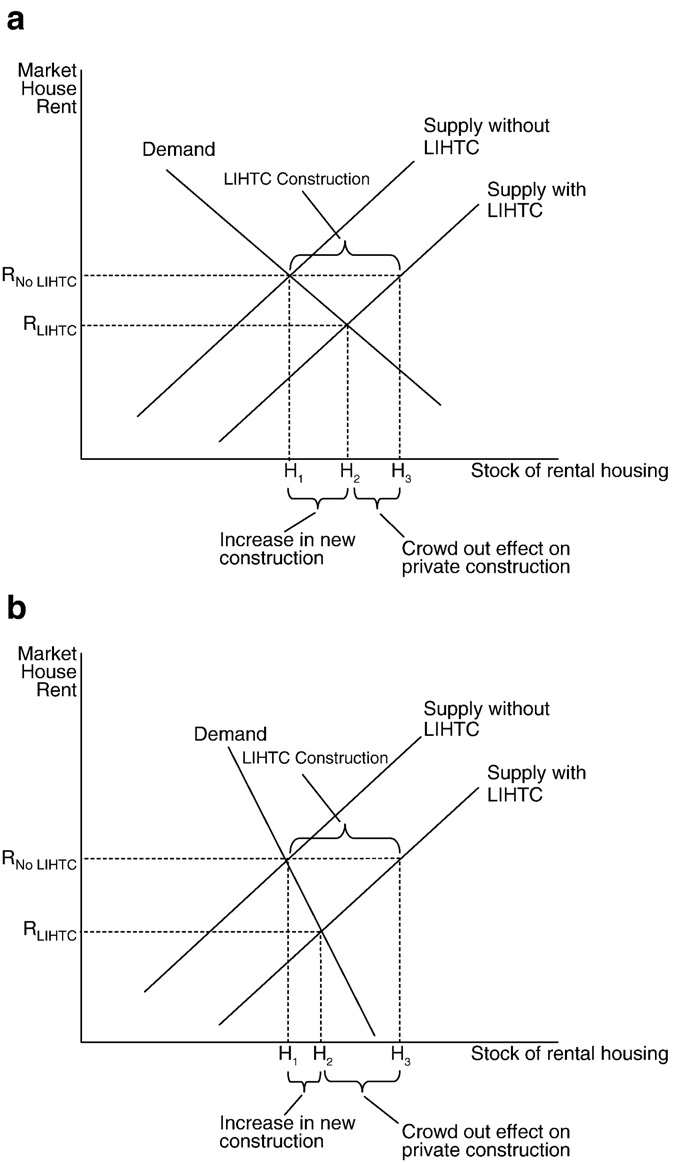
\includegraphics[width=16cm]{fig2.png}
	\caption{a: 有弹性需求的出租房被挤出,b: 因需求缺乏弹性而被挤出出租房}\label{fig2}
\end{figure}

在\figref{fig2}a中,请注意,LIHTC的开发压低了市场租金,导致出租房屋的总存量增加少于LIHTC建筑的水平($\rm{H}_2-\rm{H}_1 < \rm{H}_3-\rm{H}_1$)。不同的是,$\rm{H}_3-\rm{H}_2$表示被LIHTC项目“挤出”的无补贴私人住宅。此外,\figref{fig2}b表示随着需求函数弹性下降,挤出效应变得更加明显。事实上,只有当住房需求具有完全的弹性或者新建住房供应完全没有弹性时,$\rm{H}_3-\rm{H}_2$等于零,挤出效应才不会发生。

为了正确理解这一点,\cite{Hanushek1980449} 使用了20世纪70年代住房补贴的数据来估计出租房需求的弹性。匹兹堡(Pittsburgh)和菲尼克斯(Phoenix)的估计值分别$-$0.36和$-$0.41。对于自住住房,\cite{Rosen19791} 估计自住者随机样本的价格弹性为$-$0.99,而 \cite{Rosen19791} 估计FHA购房者的价格弹性为$-$0.5,这一群体的收入更接近于典型的租房者。这些估计证实,住房需求并非完全具有弹性。

在供给端,\cite{Mayer200085} 测算,所有类型新建住房的供给弹性大约是6,这与 \cite{DiPasquale1992337} 测算的新建多户出租住房的供给弹性为6.8十分接近。对新建住房供应弹性的其他估计较小,但通常远高于1,例如 \citep{DiPasquale1992337,Rosen19791}。虽然已有测算的供给弹性范围比需求端的变化更大,但考虑到住房存量的扩张,供给似乎也不是完全无弹性\,\footnote{从另一个角度来看,如果可开发土地充足,而实际建筑成本保持不变,那么新的住房供应应该是完全有弹性的 \citep{Rosenthal1994182}。这与住房存量的减少形成对比,因为住房的耐用性意味着供应是非弹性的 \citep{Glaeser2005345}。}。

总而言之,只有当住房需求完全具有弹性或住房供给完全没有弹性时,挤出效应才会发生。然而,文献中的测算非常明显地表明,这两种情况都不成立。除了记录在案的以中等收入家庭为目标的LIHTC计划的趋势,这表明在质量的基础上,LIHTC发展的倡导者和反对者都应该预计到该计划的挤出效应。然而问题是,挤出效应的程度是多大?

\section{数据和实证模型}\label{sec4}

\subsection{数据}

我们使用十年一次的人口普查数据作为我们控制变量的根数据源。这些数据从Geolytics公司的邻域变化数据库文件中获得的,包括1990年和2000年的数据\,\footnote{请参见 \url{http://www.geolytics.com}。}。Geolytics公司将这些年的数据重新编码到2000年人口普查区域边界,并与截至2000年投入使用的LIHTC项目的信息相结合。LIHTC的数据是通过互联网从住房和城市发展部(HUD)获得的\,\footnote{请参见 \url{http://www.lihtc.huduser.org}。}。LIHTC数据库的信息包括投入使用的年份和2000年人口普查范围,我们的数据包括17,774个LIHTC项目,共计877,972套住房。

根据这些数据,我们进行了前面提到的三组分析。在第一种情况下,所有的数据都被汇总到MSA级别,MSA是一个足够大的地理单元,因此在引言中描述的跨社区的大多数交互都应该被考虑在内。对于这一部分的分析,我们从样本中删除非MSA区域。在第二种方法中,我们将数据聚集到县一级。虽然在地理上没有MSA大,但有更多的县,这增加了数据的差异,有助于测算LIHTC的挤出效应。此外,尽管我们在MSA层面的分析中包括了州固定因子,但对于县一级的回归,我们可以使用MSA和州特定的非MSA固定因子。

对于我们的最终方法,我们使用地理信息系统(GIS)软件将数据重组为半径10英里的统一圆形单位,每个圆围绕2000年人口普查的单个地理质心$i$ ($i = 1, \dots,n$)\,\footnote{MapInfo和MapBasic用于处理数据的地理特征,在绘制人口普查中心周围的圆时,使用比例和测度来计算各种计数变量。}。所有的因变量和自变量,以及用于构建工具的总体变量,都产生了基于循环的测量。这确保了用于测量回归方程两边的变量的地理位置是相同的。值得注意的是,大部分县所覆盖的区域小于半径10英里的圆圈。由于这个原因,我们认为10英里范围内的测算至少在与县进行跨社区互动方面做得很好。此外,由于圆圈是围绕基础普查区的地理质心绘制的,因此许多不同的圆圈都位于给定的县的区域内。这使我们能够控制县级固定因子,并进一步加强识别。为了考虑圆的重叠特性和因变量中某些信息隐含的重复,我们在县一级对圆回归中的标准误差进行了聚类。州级、县级、10英里圈数据汇总统计如\tabref{tab3}所示。

\renewcommand\arraystretch{1}
\begin{table}[h]
  \centering
  \setlength{\tabcolsep}{6mm}
    \caption{回归变量的样本均值}\label{tab3}
      \begin{tabular}{lccc}
        \toprule
        & \textbf{MSA} & \textbf{县} & \textbf{10英里半径圈} \\
        \midrule
        1990--2000年私人出租住房建设量 & 8582.9 & 944.0 &
        9371.8 \\
        1990--2000 LIHTC建设量  & 1601.9 & 187.2 & 2158.6 \\
        \# 1980--1989年出租住房建设 & 15799.3 & 1704.8 &
        19027.8 \\
        \# 1970--1979年出租住房建设 & 16786.5 & 1828.5 &
        22174.7 \\
        \# 1970年以前建设的出租住房 & 42474.2 & 4798.4 &
        96303.6 \\
        \# 1980--1989年建造的自住住房 & 27004.7 & 3085.2 &
        19160.1 \\
        \# 1970年至1979年建造的自住住房 & 29625.9 & 3363.2 &
        21629.0 \\
        \# 1970年以前建造的自住住房 & 81365.0 & 9604.7
        & 111190.7 \\
        1990年的空置出租房 & 7089.0 & 816.1 & 10524.7 \\
        1990年的空置自住住房 & 2799.5 & 324.3 &
        3059.7 \\
        1990至2000年人口变化数量 ($\Delta$Pop) & 77639.0 & 8429.2 &
        102821.9 \\
        1990至2000年中位数变化 ($\Delta$Inc) & 952.4 & 111.1 &
        577.59 \\
        观测值 & 427 & 3052 & 49,794 \\
        \bottomrule
      \end{tabular}
  \end{table}

\subsection{房屋开工模型}

前面概述的理论模型描述了LIHTC发展对住房总量的影响。在这种情况下,完全挤压意味着LIHTC的建设不会对当地经济中的住房总数产生影响。\cite{Sinai20052137} 利用了这种直觉,并设计了一个模型,关注给定时间点已占用住房的总存量。我们采取不同但密切相关的方法,具体而言,以住房存量的滞后水平为条件,评估LIHTC发展对1990年至2000年间住房存量变化的影响。在这种情况下,完全挤出意味着每一套LIHTC住房的建成将减少一个单位的私人非补贴住房存量的变化。我们采用这种方法部分是因为它允许我们利用我们数据的横向优势。

我们的模型借鉴了已有的关于住房开工的相关研究,尤其是 \cite{Mayer200085} 所做的工作\,\footnote{可以参见 \cite{Topel1988718} 和 \cite{DiPasquale1992337} 获得相关信息。},他们强调,新的住房建设是流动的,因此,最好表示为住房价格和成本变化的函数,而不是这些因素水平的函数。他们还认识到,现有住房存量的恶化为新住房开发提供了进一步的动力。

Mayer and Somerville 利用美国季度总时间序列数据建立了他们的模型。$t$期和$t_1$期之间的住房开工数表示为质量调整后的房价变化、实际利率变化、建筑材料成本变化、待售住房市场滞后中值时间和现有住房存量滞后水平的函数\,\footnote{\cite{Mayer200085} 还考虑了一个AR(1)项和一个时间趋势,这有助于减少未观察到的因素的影响。如下所示,我们也考虑到了类似原因的系列相关性。}。这些控制措施的解释大多是直接的。不断上涨的房价激励开发商增加供给,而不断上涨的利率和建筑成本增加了开发成本,则减少了供给量。未售房屋在市场上待售的时间越长,表明库存增加,这可能会使开发商不愿意再建造新房。住房的初始存量越大,越多的老房子可能会变得破旧或风格过时,因此更换的时机已经成熟。较高的初始库存量,也可能反映出推动住房需求和供应的其他未观测到的因素的影响。

我们的目标是建立一个考虑到上述特征的模型,根据我们数据的性质和LIHTC计划的时间进行定制。在模型中加入LIHTC发展,可以让我们评估该项目的挤出效应。首先,我们将1990年到2000年(我们数据的时间段)之间某个给定地点的住房开工数表示如下:

\begin{equation}\label{eq4.1}
  \begin{aligned}
  s_{d}^{rental,unsubsidized}=\ & b_{1} \Delta p_{d}^{Q-adjusted}+b_{2} S_{d, 1990}+b_{3} \Delta r a t e \\
  &+b_{4} \Delta q_{r}^{Non-Landinputs}+b_{5} S_{d, 1990}^{rental, vacant}+\varepsilon_{d}
  \end{aligned}
\end{equation}
\vspace{2pt}

在公式 \eqref{eq4.1} 中,下标$d$表示所讨论的位置,而$r$是$d$所处的更广泛的地理区域。这种区别允许我们使用区域固定因子来控制一些变量,正如前面所提到的,稍后将会阐述。前面我们用三种不同的方式来编码地理位置,最初,我们让$d$表示一个给定的MSA,在这种情况下,我们将县所在的州视为更广泛的区域,用$r$表示。对于跨越州边界的多州行政区,我们将多州行政区划分为与组成州中的那些区域相对应的部分,并将每个部分视为单独的对象。在我们的第二种方法中,$d$表示给定的县。在这种情况下,我们将县所在的MSA视为更广泛的区域,前提是该县在MSA中。对于不在MSAs中的县,$r$被编码为该县所在的州。在最后的方法中,$d$被设置为半径为10英里的圆,$r$被设置为圆的地理中心所在的县。

以这种方式定义$d$和$r$允许我们控制上面提到的房屋开工的潜在驱动因素。需要说明的是,因变量$s_{d}^{rental,unsubsidized}$是指1990年至2000年间未被补贴的出租房数量,而$S_{d,1990}$是指1990年住房(租金加自有住房)的滞后总数。如前所述,$S_{d, 1990}$控制了许多未观测到的项,也确保了我们的因变量反映了不同时期住房存量的变化。同时,$S_{d, 1990}^{rental, vacant}$是指1990年空置出租住房的数量,并考虑到当年可能出现的不平衡情况。这些变量都随着$d$的变化而变化,并且都可以很容易地使用前文提到的根普查区域数据,对每一种地理层次进行测量。

为了进一步充实我们的模型,我们将$S_{d,1990}$分解为在20世纪80年代、70年代和1970年之前建造的房屋的独立的部分,并且还包括针对房屋出租和业主自用库存进行独立测算。因此,我们把公式 \eqref{eq4.1} 写成下面这样:

\begin{equation}\label{eq4.2}
\begin{aligned}
  s_{d}^{rental,unsubsidized}=\ & b_{1} \Delta p_{d}^{Q-adjusted}+b_{2,1}^{rent} S_{d, 1990}^{rent, 80 t o 90}+b_{2,2}^{rent} S_{d, 1990}^{rent, 70 to 80} \\
  &+b_{2,3}^{rent} S_{d, 1990}^{rent, pre 70}+b_{2,1}^{own} S_{d, 1990}^{own, 80 to 90}+b_{2,2}^{own} S_{d, 1990}^{own, 70 to 80} \\
  &+b_{2,3}^{own} S_{d, 1990}^{own, pre 70}+b_{3} \Delta rate+b_{4} \Delta q_{r}^{Non-Landhputs} \\
  &+b_{5} S_{d, 1990}^{rental,vacant}+\varepsilon_{d}
  \end{aligned}
\end{equation}

公式 \eqref{eq4.2} 包括1990年出租和自住住房存量住户的年龄分布,相比公式 \eqref{eq4.1},在某种程度上,未被观察到的本地房屋开工驱动因素是连续相关的,因此,上世纪80年代开发的与房屋相关的术语将倾向于吸收这种影响(例如$S_{d, 1990}^{rent, 80 to 90}$)。实际上,我们允许一个AR(1)过程,就像 \cite{Mayer200085} 一样进行处理。与此同时,1990年的旧住房存量(如1970年以前建造的住房,$S_{d, 1990}^{rent, pre70}$)将遭受更大程度的恶化。这些股票更有可能被替换,它们的存在可能导致20世纪90年代更多的住房开工。租房和自住住房也很可能只是较弱的替代品,在这种情况下,我们预计与自住住房相比,滞后租房会产生更强的影响。

公式 \eqref{eq4.2} 中的其余项中,$\Delta rate$表示实际利率的变化,是最容易考虑的,这个变量被认为在20世纪90年代在所有地方都很常见,当我们使用单个横截面进行估算时,$\Delta rate$在方程中 \eqref{eq4.2} 中是一个常数。$\Delta q_{r}^{Non-Landhputs}$是非土地要素投入代表。重要的是,我们假设这个变量在不同的区域是不同的,但是在给定的$r$内是恒定的,作为一个近似值,这似乎是合理的。给定这个假设,我们可以通过在模型中包含区域固定因子来消除$\Delta q_{r}^{Non-Landhputs}$的影响。

剩下的只有$p_{d}^{Q-adjusted}$,表示$d$区域内质量调整后的房价在1990-2000年间的变化。如果在给定区域内房价增长差不多,那么在模型中包括区域固定因子也将使该变量有所不同。然而,出于两个原因,这不是一个非常合理的假设。首先,即使在定义的较广区域内,需求冲击在各个位置之间也可能不同,尤其是当$d$相对于$r$较小时(例如,当$d$设置为MSA且$r$在该区域内时)。其次,由于空缺率的不同,1990年不同地点的短期失衡状态可能不同。这将进一步加剧地方层面的房价在90年代变化的程度的差异。我们通过下面的调整,对$p_{d}^{Q-adjusted}$进行改进,解决了这个问题:

\begin{equation}\label{eq4.3}
  \begin{aligned}
    \Delta p_{d}^{Q-adjusted} \approx \ & a_{1} \Delta Pop_{d}+a_{2} \Delta Med \ln c_{d}+a_{3} \Delta P o p_{d} \cdot S_{d, 1990}^{rental,vacant} \\
    &+a_{3} \Delta M e d \ln c_{d} \cdot S_{d, 1990}^{rental,vacant} \cdot+a_{4} D_{d}+\delta_{r}
    \end{aligned}
\end{equation}
\vspace{2pt}

在公式 \eqref{eq4.3},区域固定因子$\delta_{r}$表示质量调整后的房价的区域变化,其余变量反映了个别地区平均效应的偏差,$\Delta Pop_{d}$指1990年至2000年间$d$区域人口的变化,同样,$\Delta Med \ln c_{d}$表示$d$区域家庭收入中位数的变化。这些因素推动了需求的变化,会对当地房价的变化产生积极的影响。这种情况的发生可能与1990年的空置住房数量有关,当大量空置住房存在时,填补空置住房至少可以部分缓解正面需求冲击,这将缓解价格上涨压力。因此,公式 \eqref{eq4.3} 中的交互项会价格产生负面影响。需求冲击也可能随着给定地点离市中心的距离而发生系统性地变化,这是因为随着时间的推移,城市倾向于从中心向外发展,然后再发展 \cite{Brueckner2009725}。考虑到这种模式,在模型中,变量$D_d$表示在模型中到市中心的距离,其中地理单位用10英里半径的圆来测量,而当我们使用MSA级别或县级数据时,则表示密度(住房套数除以土地面积)。\!\footnote{在循环回归中,我们将分析限制在MSAs的人口普查区域,并将城市中心定义为2000年人口密度最高的人口普查区域的地理质心。}。

将公式 \eqref{eq4.3} 代入公式 \eqref{eq4.2}中,对部分变量进行重新排序,我们得到:

\begin{equation}\label{eq4.4}
  \begin{aligned}
    s_{d}^{rental, unsubsidized}=\ & b_{1}^{rent} S_{d, 1990}^{rent, 80 t o 90}+b_{2}^{rent} S_{d, 1990}^{rent, 70 t o 80}+b_{3}^{rent} S_{d, 1990}^{rent, p r e 70} \\
    &+b_{3}^{own} S_{d, 1990}^{own, 80 t o 90}+b_{4}^{own} S_{d, 1990}^{own, 70 t o 80}+b_{5}^{own} S_{d, 1990}^{own, p r e 70} \\
    &+b_{6} S_{d, 1990}^{rent a l, vacant}+b_{7} \Delta P o p_{d}+b_{8} \Delta MedInc_{d} \\
    &+b_{9} \Delta Po p_{d} \cdot S_{d, 1990}^{rental, vacant}+b_{10} \Delta MedInc_{d} \cdot S_{d, 1990}^{rent a l, vacant} \\
    &+b_{11} D_{d}+\lambda_{r}+\varepsilon_{d}
    \end{aligned}
\end{equation}
\vspace{2pt}

表达式 \eqref{eq4.4} 刻画了与大部分的住房开工模型相关的主要特征\,\footnote{请注意,\eqref{eq4.3} 中的$\lambda_{r}$是所有地区特定的影响因子,包括实际利率的变化、非土地要素价格投入的变化以及价格变动的共同组成部分的变化。}。将1990年至2000年间建造的LIHTC住房数量(记为$s_d^{LIHTC}$)相加,得出我们的估算公式:

\begin{equation}\label{eq4.5}
  \begin{aligned}
    s_{d}^{rental,unsubsidized}=\ & \theta s_{d}^{LIHTC}+b_{1}^{rent} S_{d, 1990}^{rent, 80 to 90}+b_{2}^{rent} S_{d, 1990}^{rent, 70 t o 80} \\
    &+b_{3}^{rent } S_{d, 1990}^{rent , pre 70}+b_{3}^{own} S_{d, 1990}^{own, 80 to90}+b_{4}^{own } S_{d, 1990}^{own, 70 to 80} \\
    &+b_{5}^{own} S_{d, 1990}^{own,pre70}+b_{6} S_{d, 1990}^{rental,vacant}+b_{7} \Delta P o p_{d} \\
    &+b_{8} \Delta M e d h c_{d}+b_{9} \Delta P o p_{d} \cdot S_{d, 1990}^{rental, vacant} \\
    &+b_{10} \Delta M e d \ln c_{d} \cdot S_{d, 1990}^{rental, vacant}+b_{11} D_{d}+\lambda_{r}+\varepsilon_{d}
    \end{aligned}
\end{equation}
\vspace{2pt}

在这个表达式中,$\theta$是主要的变量。如果其系数等于0,则表明LIHTC住房的建设对1990年至2000年期间建造的私人、无补贴出租住房的数量没有影响。相反,如果$\theta$等于$-$1,这意味着完全挤出,表明LIHTC建设几乎没有增加租赁住房的总存量。

\subsection{内生变量}

公式 \eqref{eq4.4} 中的两组变量似乎特别倾向于内生性。第一个是关键控制变量:LIHTC项目的住宅开发。第二个是对1990年至2000年间$d$区域人口和收入中位数变化的控制,我们首先考虑后者。

在特定地点建设新住房有可能吸引住户,而建造出租住房尤其吸引低收入家庭。出于这两个原因,一个地区的人口和收入中位数的变化可能是新住房开发的内生因素。为了解决这一问题,我们通过将$d$区域1990年的人口(中位收入)乘以更广泛地理区域的人口(中位收入)增长百分比来衡量$d$区域内的人口(中位收入)变化:对于MSA级和县级模型,乘以州级人口和中位收入的百分比变化,而对于10英里环形模型,乘以MSA层级人口和中位收入的百分比变化。在每种情况下,我们都做了两个假设:(I)$d$区域1990年的人口和中位收入水平在1990--2000年间的住房发展是外生的,(ii)更广泛区域的人口和中位收入的百分比变化对$d$区域90年代的新住房建设是外生的。第一个假设实际上与假设1990年的住房存量是外生的没有区别,这个假设已经隐含在住房开工模型 \eqref{eq4.1} 中。第二个假设相当于认为,一个小的地理单位的发展不会显著影响一个大得多的地理区域的人口和收入的总体增长率。

采用不同的策略来控制LIHTC住房的可能的内生布局。如前言所述,我们使用LIHTC发展工具,通过两阶段最小二乘法来评价模型,这些工具是由管理LIHTC信贷分配的政治进程所驱动的。第一个工具是通过将一个地区例如县1990年在该州人口中所占的份额,乘以该州在90年代对LIHTC信贷的分配而获得。这模拟了联邦政府依据各州在全国人口中所占的比例进行信贷分配的过程。第二个工具基于给定地区是否在1989年投票给现任州长,使用1–0虚拟变量进行表示\,\footnote{1985年至1988年的州长选举结果是根据1950年至1990年由政治和社会研究大学间联合会(ICPSR)编制的美国大选数据系列得出的。}。对于MSA回归,1–0投票虚拟变量是针对给定MSA的每个州特定部分单独测算的;对于县级回归,虚拟变量基于县级投票模式进行编码;对于半径为10英里的圆形回归,使用与圆形地理质心所在的县相对应的县一级投票结果。以这种方式对第二个工具进行编码,并考虑到任人唯亲的可能对宝贵的LIHTC补贴的影响。

\subsection{重叠圆圈}

最后一个实证问题是当$d$被设置为10英里半径的圆区域时,圆的重叠情况。因为圆形测量是围绕基本人口普查区域的地理质心绘制的,所以附近的圆圈通常会重叠。这表明我们的因变量依赖于重叠的信息,而不是独立的。这个问题不解决将导致模型标准误差向下偏移,但不会偏移系数估计值。为了解决这个问题,在圆周上测量变量时,我们将标准误差集中在县一级。

\section{实证分析结论}\label{sec5}

\tabref{tab4}根据前面描述的MSA、县和10英里环形地理,给出了三组挤出回归的OLS和2SLS估计值。在所有情况下,我们的因变量是1990年至2000年间建造的私人出租住房的数量。固定因子与前面描述的分析基础的地理水平不同,并在表格底部注明。还要注意的是,对于县一级的回归,我们在完全由单一县组成的管理服务协议中删除了县;对于10英里圆回归,我们将样本限制为质心位于移动平均线的圆单位\,\footnote{我们将样本限制在MSAs内的位置是出于两方面的原因。一是MSAs潜在的人口普查区更小,这有助于减少将数据重新编码为圆形时的测量误差。二是MSAs拥有定义好的中心,可以将到MSA中心的距离作为控制变量放弃,非MSA的县对结果几乎没有影响。}。在所有情况下,模型估计的标准误差都集中在固定因子所用的同一地理水平上。

\begin{table}[h]
  \caption{1990年至2000年的私人出租建设(括号内是$t$的比率)}\label{tab4}
	\centering
	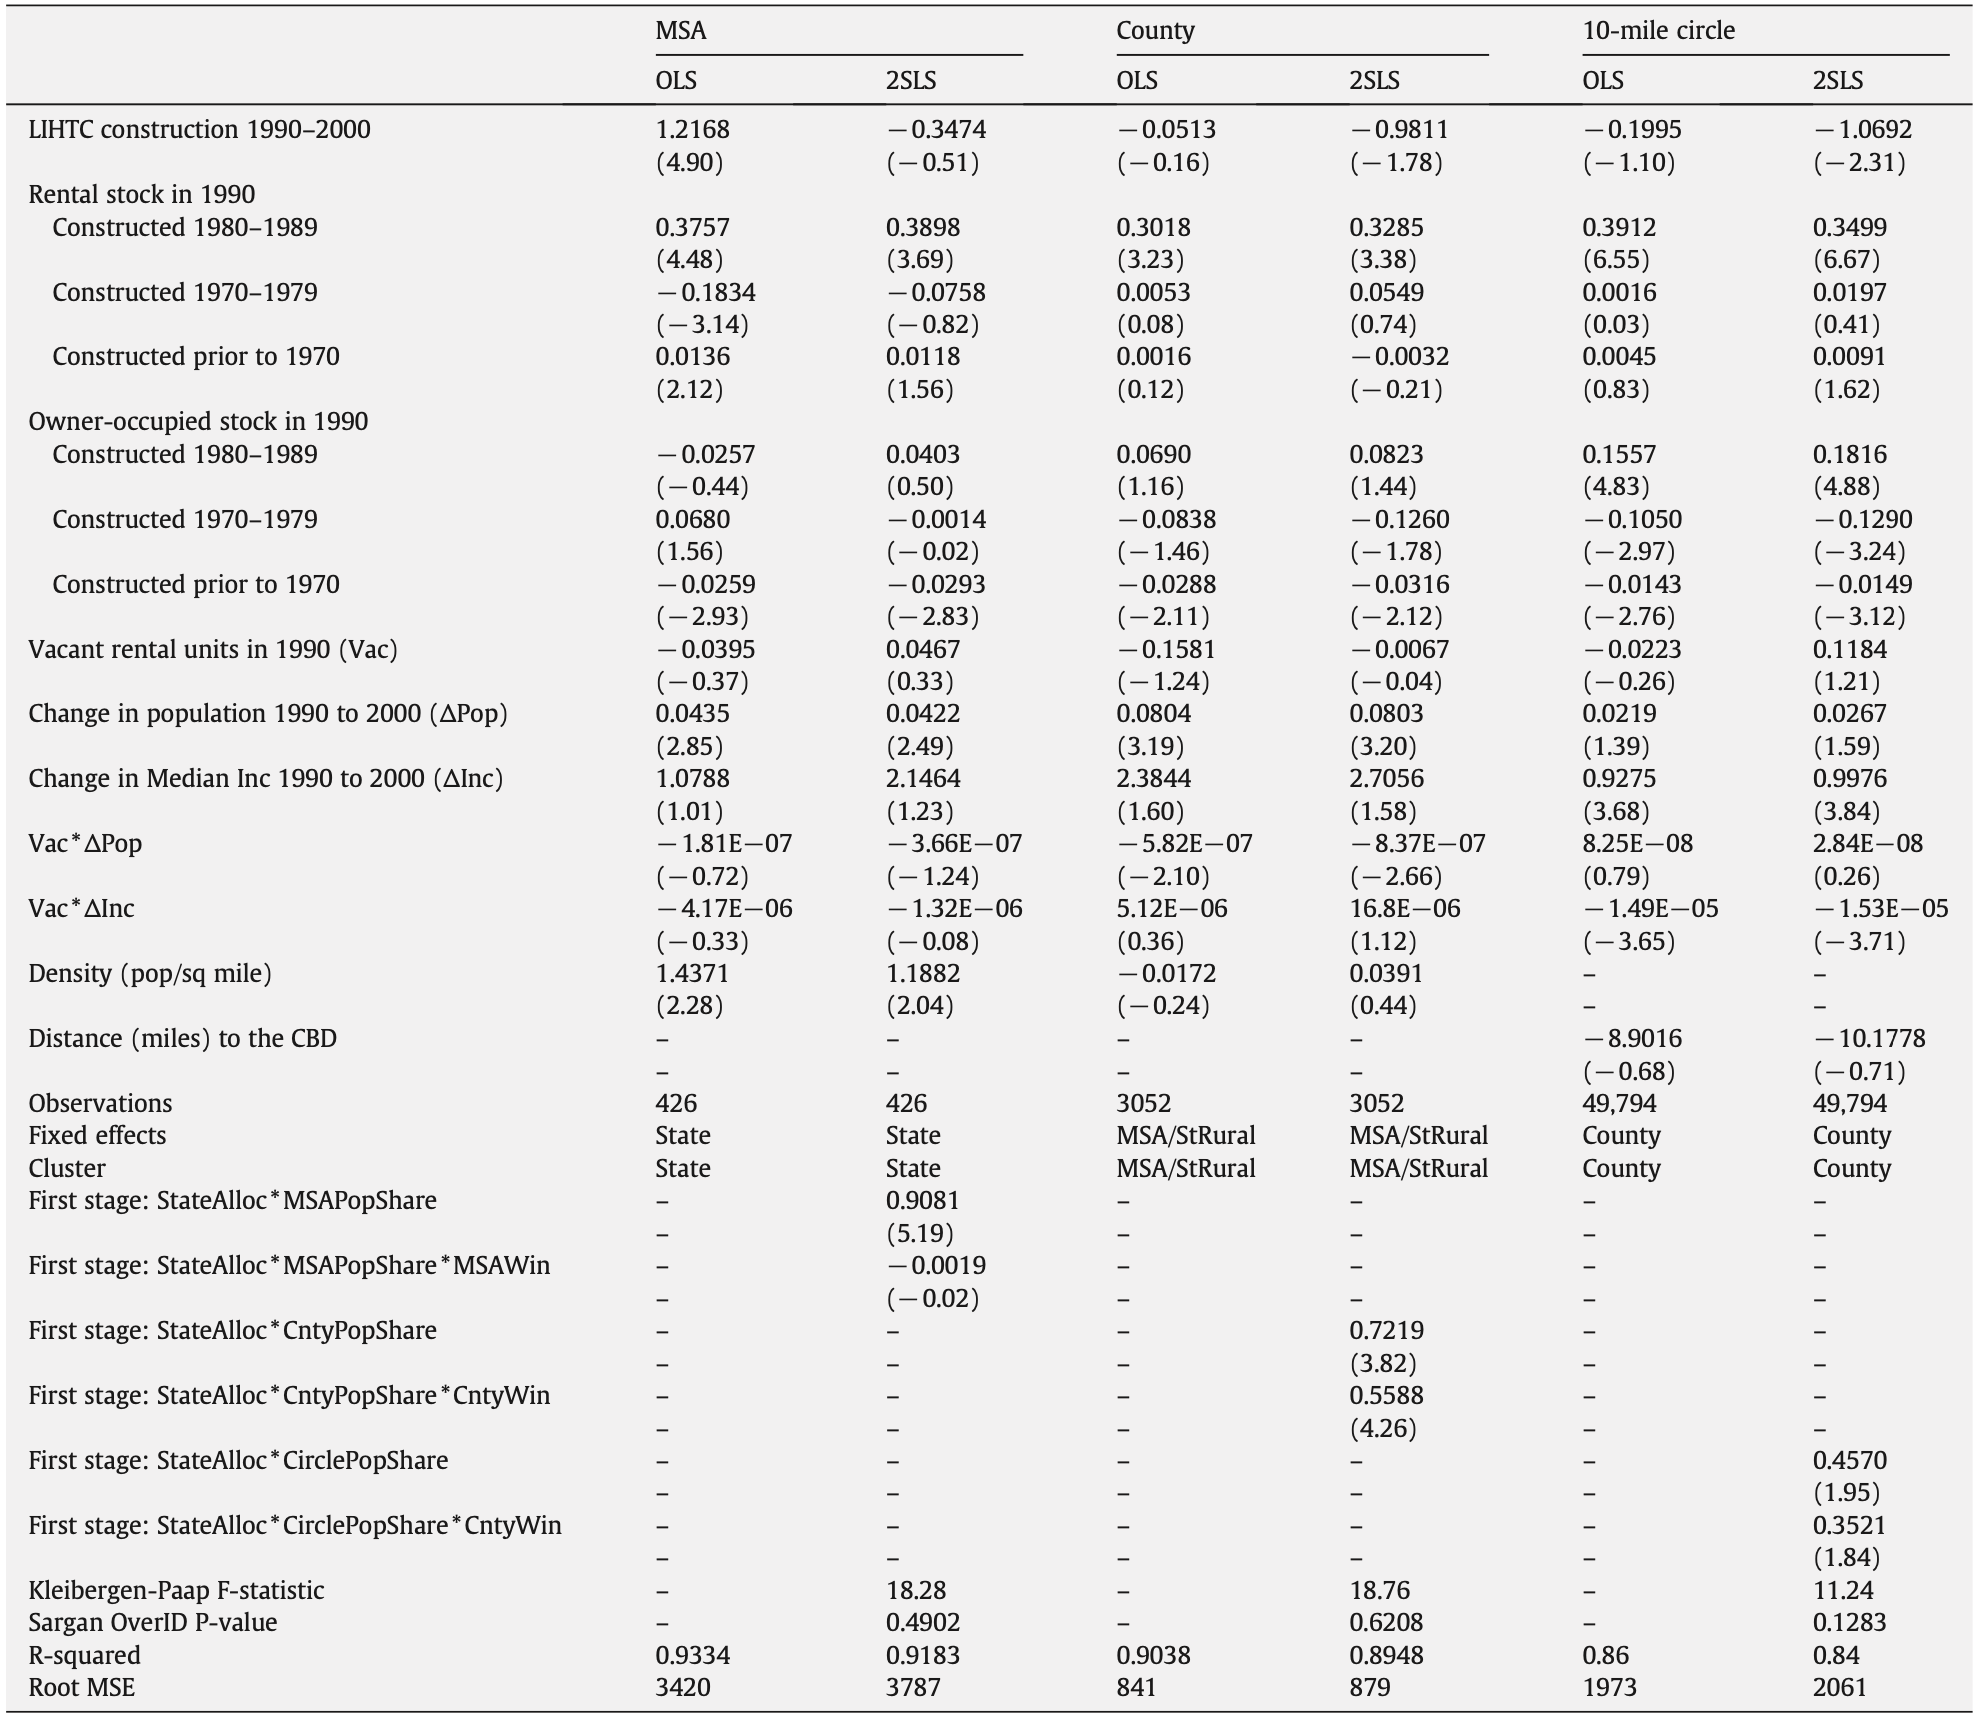
\includegraphics[width=17cm]{tab4.png}
\end{table}
  
首先考虑\tabref{tab4}中关于LIHTC开发以外的系数。在每一列中,无论LIHTC是外生的(使用OLS)还是内生的(使用2SLS),这些变量的系数差异都非常小。更令人震惊的是,租金和自有住房的滞后存量的系数对基本地理分析单位并不特别敏感。最极端的例子是80年代建造的出租房屋,其在所有不同模型中的系数在0.3到0.4之间。这种模式表明,随着人们改变分析的地理单位:(i)因变量和自变量的变化比例大致相等,并且(ii)滞后的住房存量与新开工建筑之间的关系在不同规模的地理单元上是相似的。

对滞后住房存量变量的更仔细的研究表明,在出租房屋开工中,一阶序列相关性很强。例如,考虑\tabref{tab4}中从右数第二列到最后一列的10英里圆回归的估计值,在1990年的出租住房中,80年代建造的单元的系数为0.39,$t$比率为6.55,对于70年代建造的出租住房和1970年之前建造的出租住房,相应的系数接近于0,在统计上不显著。还要注意,对1990年自有住房存量的相应估计较小:例如80年代建造的单元的系数仅为0.16,$t$比率为4.83。这些模式表明,在20世纪80年代促成住房建设的未被注意到的趋势,往往会持续到90年代。此外,正如所料,与现有自有住房存量相比,租赁住房建设对现有租赁住房存量更为敏感。这与住房市场在出租和自住部门之间严重分割的观点是一致的。这进一步表明,LIHTC建设对非补贴开发的影响可能在房屋市场的租赁领域最为明显,而不是业主自住领域,我们将在后文再次讨论这一点。

接下来观察到,人口和收入中位数的变化都与90年代对出租房屋的建设产生了积极影响。对于10英里OLS模型,对于人口,系数为0.0219,$t$值为1.39; 对于中位数收入的变化,系数为0.93,$t$值为3.68。此外,虽然人口变量与租金空缺之间的相互作用不够明显($t$值为0.79),但收入变量的相互作用为负且很明显,$t$值为$−$3.65。这些结果表明,至少在收入方面,租赁房屋的建设增加,但幅度不大,以至于1990年空置租赁住房的数量增加了\,\footnote{90年代人口和收入中位数变化的系数,以及它们与1990年空缺率的相互作用,确实与地理分析水平有所不同。然而,广泛的模式下是稳健的。}。这与假设相符合:收入和人口推动需求上升,建筑量增加,但若有空置住房,则比例比较低。

现在考虑一下1990年代LIHTC开发对无补贴建筑的影响\,\footnote{非LIHTC变量上的其余系数在很大程度上是不重要的,因此特别没有强调。例如,请注意,尽管在OLS模型中,空置率具有进一步的直接负面影响(系数为0.158,$t$比率为1.24),但在将LIHTC住房视为内生住房时,该系数几乎为零。此外, \tabref{tab4}中的任何模型都没有证据表明密度有明显的影响。}。我们从OLS的估计开始,对于MSA、县和10英里圆回归,LIHTC发展系数为 $+$1.2(t比率为4.90)、0.05($t$比率为0.16)和0.199($t$比率为1.10)。从表面上看,OLS的估计未能提供LIHTC挤出效应的证据。然而值得注意的是,随着模型中包含的地理水平和潜在固定效应变得更加精确,LIHTC发展的OLS系数负得越多:对于具有州级固定效应的MSA级回归,为正1.2;对于具有MSA/州-农村固定效应的县级回归,为0.05;对于具有县级固定效应的10英里循环回归,为0.199。这表明,未能充分控制当地未观察到的建筑驱动因素会使LIHTC系数偏向一个更加大的正数。这与LIHTC和未受资助的开发项目都被吸引到具有未被观察到的有利可图属性的地区的想法是一致的。

将OLS与LIHTC系数的2个最小二乘估计值进行比较,进一步说明了这一观点。对于每一个地理层级,2SLS对LIHTC系数的估计都要负得多:MSA级回归为0.35($t$比率为0.51),县级回归为0.98($t$比率为1.78),10英里圆回归为1.07($t$比率为2.31)。相对于OLS,这些估计证实了OLS模型的上升趋势(更积极的)偏差。这进一步表明,开发商倾向于将LIHTC项目定位于已经在进行无补贴开发的增长区域,虽然这种模式不是挤出发生的必要条件,但它肯定与预期一致。

最后,估计挤出效应的程度非常重要。为此,我们强调10英里圆圈模型,它是基于上述原因(例如更精确的地理固定效果)的最可靠的回归。对于这种模式,我们的点估计表明,LIHTC的发展完全被新出租住房的无补贴发展的减少所抵消,尽管置信区间足够宽,以允许更适度的影响,但在阐述之前,需要进一步说明。

\subsection{分析优势与有效性}

\tabref{tab4}的底部报告了仪器的诊断统计数据以及第一阶段仪器系数。附录中\tabref{taba-1}报告了完整的第一阶段回归。鉴于我们对10英里圆回归的偏好,我们强调对该规格的诊断。尽管基于不同基础地理分析单元的模型在诊断方面存在一些差异,但大多数情况下模式是相似的。

对于10英里圆回归,请注意所包含的工具的第一阶段系数是正的,并且个别显著,t比率分别为1.95和1.84。正系数如预期的那样:投票支持获胜州长候选人的人口更多的地区和县将获得更多的LIHTC学分和相关建设拨款。仪器系数的统计显著性也表明模型至少被识别。重要的是,作为一对,这两种工具与内生变量密切相关,如Kleibergen-Paap F-统计值11.24所示。该值高于通常用于评估弱仪器偏差是否是一个严重问题的“10”,例如 \cite{Stock200580}。总的来说,我们得出结论,我们的工具似乎有预期的迹象,而且我们的估计不太可能受到弱工具偏差的影响\,\footnote{对于允许标准误差为异方差的情况,弱仪器测试的临界值还有待开发,如聚类标准误差,可参见\cite{Stock200580}。然而,\tabref{tab4}底部的证据表明,弱仪器偏差不是问题。}。

原则上,也可以测试第四列中的过度识别限制是否可以被拒绝。这种证据可能表明模型的错误描述,包括工具可能是内源性的。对于10英里圆回归,萨甘测试的结果表明P值为0.1283,这不能拒绝模型和仪器被正确指定的空值。然而,我们警告说,众所周知,萨甘测试对型号规格很敏感,而且能力很弱。当工具与内生变量相关的机制相似时,尤其如此,因为两种工具都利用人口份额 \citep{Cameron2006,Murray2006111}。

假设所有的工具都是有效的,那么使用工具子集的估计应该产生渐近相似的估计。\tabref{tab5}探讨了这个想法。第1列和第4列重复\tabref{tab4}中提供的OLS和2SLS估计,以方便比较,而第2列仅使用人口共享作为工具提供2SLS估计,而第3列仅使用任人唯亲变量作为工具。

\begin{table}[h]
  \caption{1990年至2000年期间,在10英里环形水平上,使用不同的工具组合(圆括号中的$t$比率)进行竞争租赁建设。}\label{tab5}
  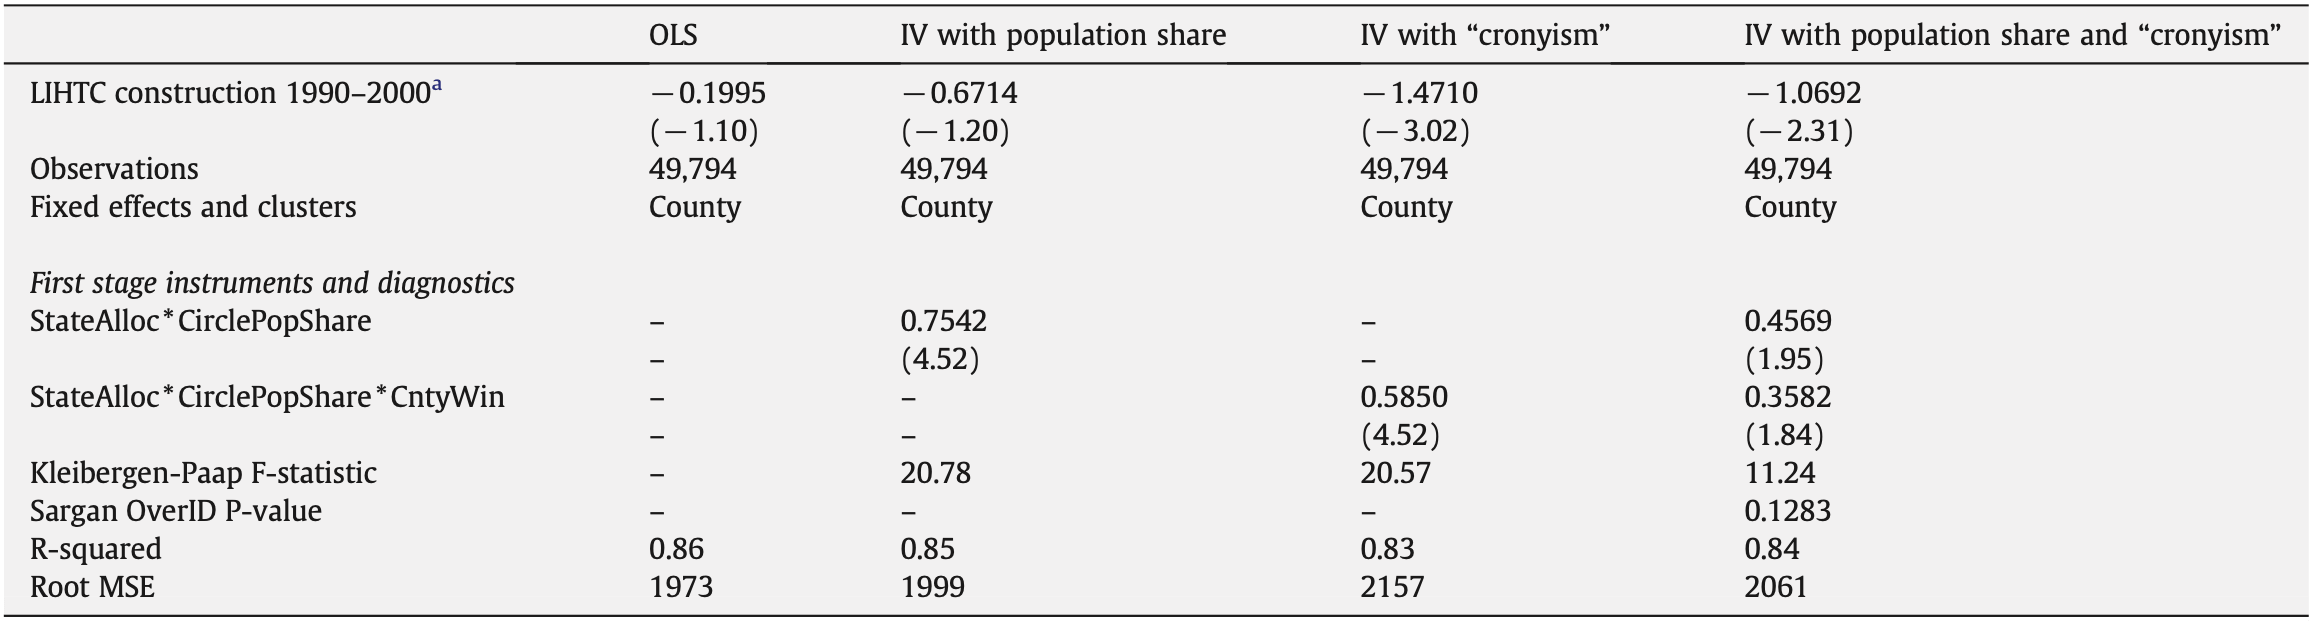
\includegraphics[width=17cm]{tab5.png}
\noindent\;{\scriptsize $^\text{a}$ 其他控制变量如\tabref{tab4}所示,但没有报告以节省空间。}
\end{table}

对于\tabref{tab5}的中间两列,请注意,当使用人口份额作为工具时,LIHTC系数等于 −0.67($t$比率为1.20),而当裙带关系变量为−1.47(t比率为3.02) 而是用作乐器。 当两个工具都包含在第一阶段中时,LIHTC系数等于 -1.07,如先前报告的那样。 此外,很明显,当在中间两列中单独使用这两种工具时,每种工具都具有非常显着的正系数,因此与内生变量密切相关(请注意,Kleibergen-Paap F统计量远高于10) 。 更一般而言,尽管各个模型的LIHTC系数估算值显然存在差异,但所有三个2SLS模型都指向同一方向:证据继续表明,LIHTC的发展在很大程度上被无补贴的私人租赁建筑的置换所抵消。

\subsection{业主自用建筑}

在前面的讨论中,我们注意到,\tabref{tab4}中的证据表明,与自有住房的现有存量相比,未补贴的租赁住房建设与给定地区现有租赁单元的构成关系更为密切。这表明但没有证实LIHTC的发展将对市场的租赁方面产生更大的替代效应。我们在\tabref{tab6}中考虑了这个问题。

\begin{table}[h]
  \caption{对于不同的细分市场(圆括号中的t比率),在10英里圆的水平上挤出效应。}\label{tab6}
  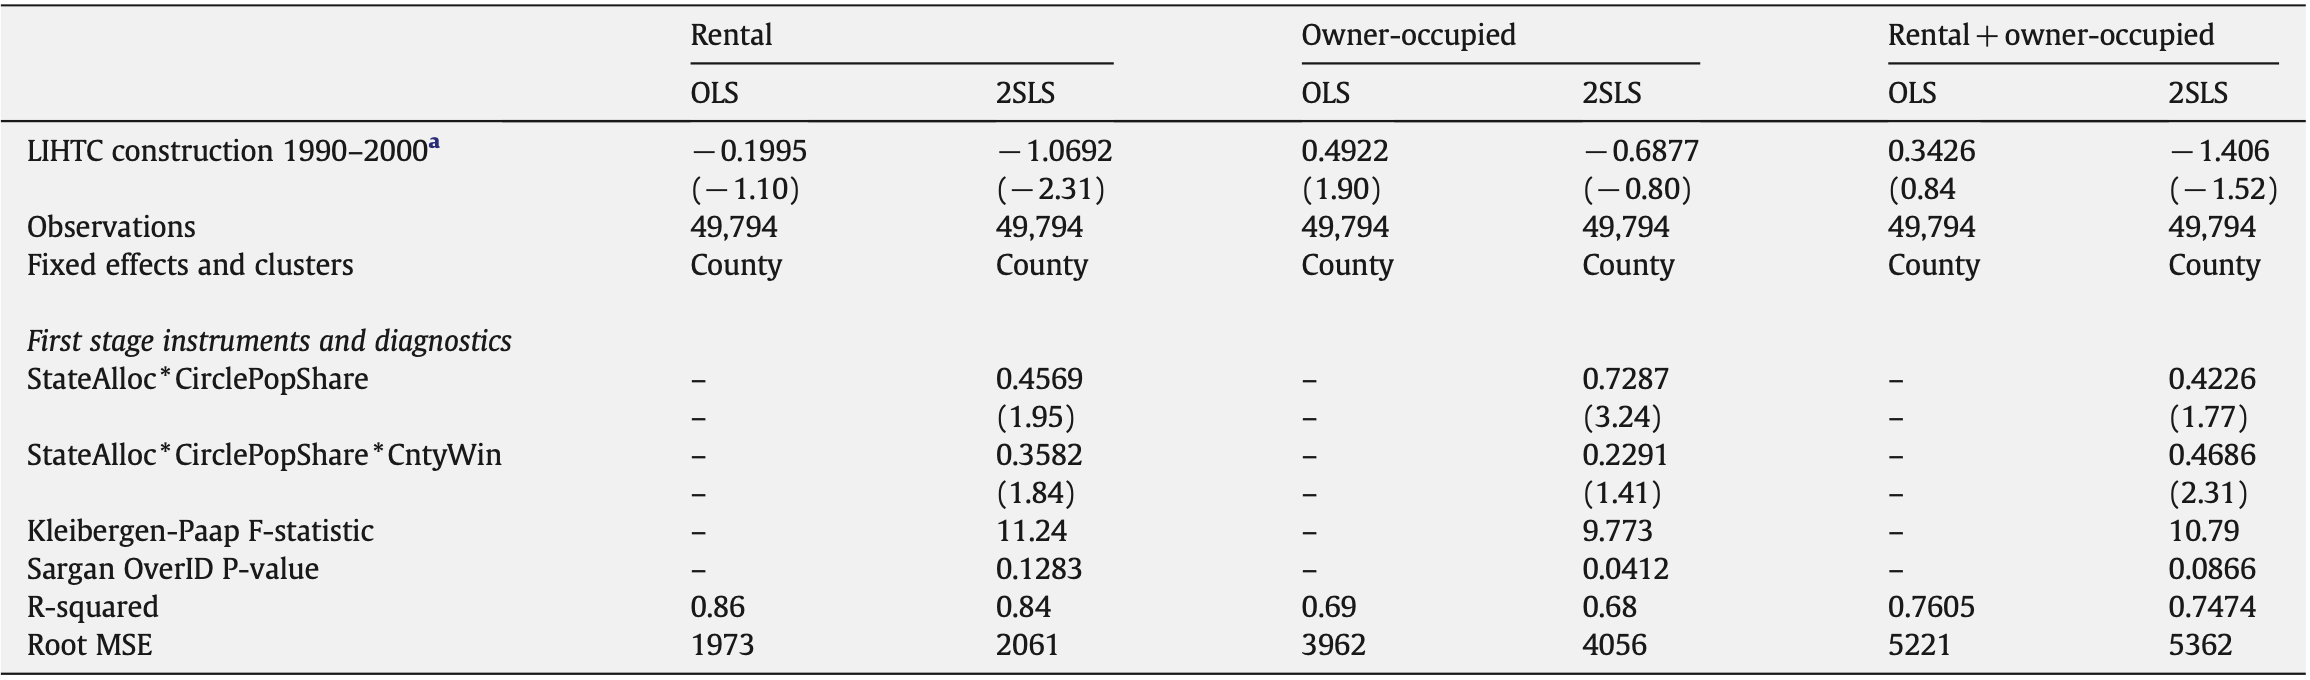
\includegraphics[width=17cm]{tab6.png}
\noindent\;{\scriptsize $^\text{a}$ 其他控制变量如\tabref{tab4}所示。完整的回归结果见附录\tabref{taba-2}。}
\end{table}

\tabref{tab6}给出了LIHTC对三组OLS和二次最小二乘10英里圆回归的挤出估计。第一个是\tabref{tab4}中对私人租赁建筑的估计,再次重复。第二次使用20世纪90年代建造的自住住房作为因变量。第三种方法是将20世纪90年代私人租赁加自住建筑的总和作为因变量。对于后两种模型,回归中的空置率分别基于业主自住和租金加业主自住的空置率。该模型的所有其他特征与之前一样,其他模型系数在表6中被抑制,以便将注意力集中在LIHTC系数上。附录的\tabref{taba-2}中列出了这些附加模型的完整估计值。

在\tabref{tab6}中,请注意,对于每组回归,OLS得出的正估计数远远多于2LS:对于自有住房和租赁加自有住房模型,OLS系数分别为正0.49(t比率为1.90)和正0.34($t$比率为0.84)。这些模型的相应2SLS估计值分别为0.6877和1.4。证据再次表明,控制LIHTC发展的未观察到的驱动因素的重要性,否则将使LIHTC系数偏向一个更积极的值。

还应注意,与租赁行业相比,业主自用行业的2SLS LIHTC系数更小、更不精确:业主自用行业为0.68,标准误差为0.86(t比0.8),而租赁行业为1.07,标准误差为0.46(t比2.31)。当合并两个扇区时,LIHTC点估计的幅度较大(1.406),但相应的标准误差也很大(0.93),导致t值为1.52。总的来说,这些结果提供了有限的证据表明,LIHTC的发展可能取代建设业主自用的单位。相反,与\tabref{tab4}中的模式相一致,这里的证据表明,LIHTC建设的挤出效应可能主要是通过无补贴的租赁住房建设的转移而产生的。

\section{结论}\label{sec6}

\begin{figure}[t]
	\centering
	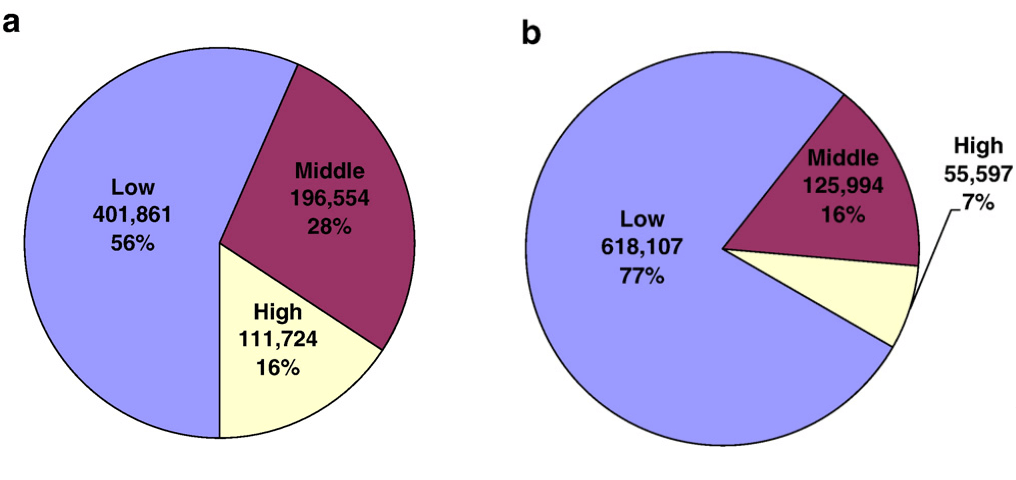
\includegraphics[width=14.2cm]{fig3.png}
  \caption{a: 按2000年居民收入状况划分的低收入住房税收抵免住房,b: 按2000年居民收入状况划分的传统公共住房的位置}\label{fig3}
\end{figure}

最近低收入住房税收抵免(LIHTC)计划的急剧增长,使一个老问题获得了新的重要性。政府应该通过租户或安置项目提供低收入住房支持吗?在这种背景下,LIHTC项目自1987年启动以来迅速发展,现在是美国历史上最大的补贴租赁住房建设项目。该项目为符合条件的项目补贴了30\%至91\%的建设成本,近年来已占到所有多户租赁住房建设的三分之一。此外,国会最近的提案试图将该项目规模扩大一倍。然而,人们对这个日益重要和昂贵的项目的效果知之甚少。本文试图填补这一空白。

我们最重要的发现是,由于LIHTC计划,私人租赁住房建设的转移是巨大的。我们最可靠的点估计表明,几乎所有LIHTC的发展都被挤出未补贴的租赁住房建设抵消了,尽管这一估计的置信区间允许更适度的影响。进一步的分析未能提供令人信服的证据证明LIHTC的发展影响了自住单元的建设。这似乎证实了LIHTC转移效应主要出现在住房市场的租赁部门。

这些发现表明,LIHTC计划的支持者需要超越简单地扩大出租房屋的总体存量来证明该计划的持续性。一种可能性是,LIHTC的发展可能会影响到中低租金住房机会的所在地。例如,\figref{fig3}a中的汇总措施表明,截至2000年,77\%的公共住房单元位于低三分之一收入地区,其余大部分位于中三分之一收入社区。与此形成鲜明对比的是,\figref{fig3}b显示,截至2000年,16\%的LIHTC单位位于其生活津贴收入分布的上三分之一的人口普查区域,而另外28\%位于中等收入社区(其余56\%位于低三分之一收入社区)。LIHTC住房向中三分之一和高三分之一收入社区的延伸,与过去的公共住房项目截然不同。这也增加了LIHTC发展可能帮助低收入和中等收入家庭获得更高质量的当地学校和其他当地公共服务的可能性。我们把这个作为进一步研究的领域。

\appendix
\setcounter{table}{0}
\renewcommand\thetable{A-\arabic{table}}
\section*{附录}

\begin{table}[h]
  \caption{LIHTC建设的第一阶段估计(圆括号中$t$比率的绝对值)。}\label{taba-1}
  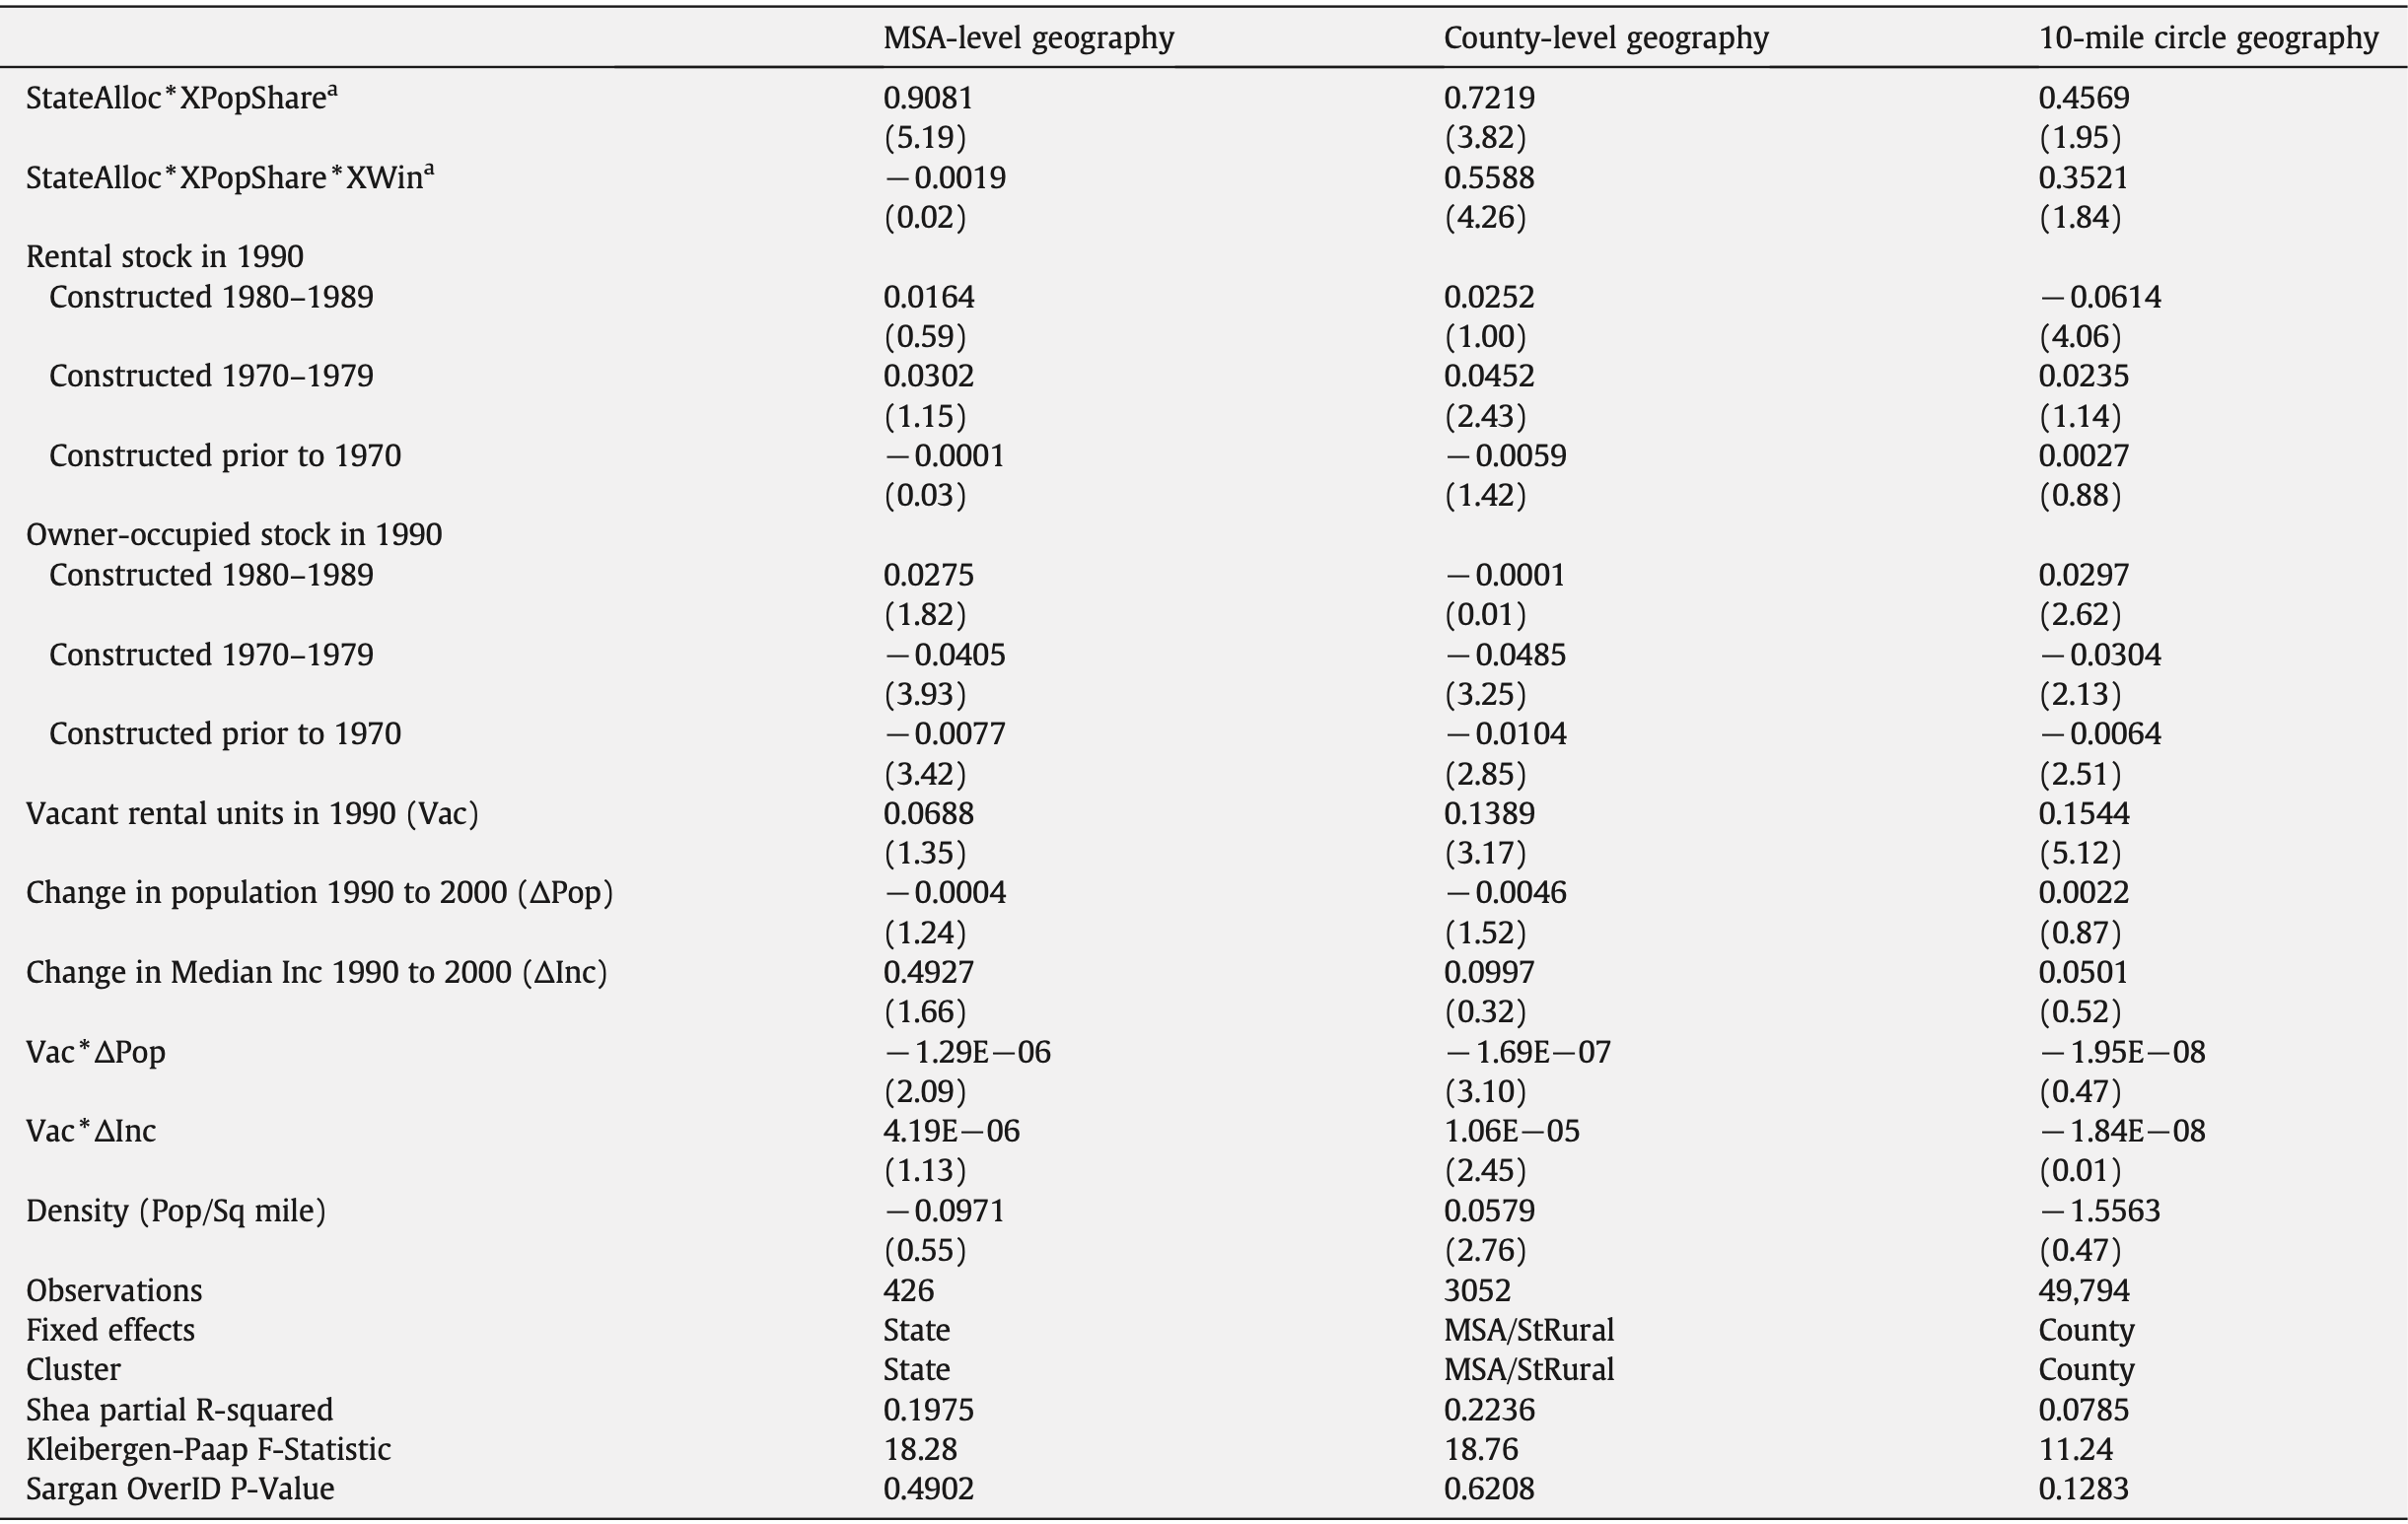
\includegraphics[width=17cm]{taba-1.png}
\noindent\;{\scriptsize $^\text{a}$ LIHTC建设的第一阶段估计(括号中$t$比率的绝对值)。}
\end{table}

\begin{table}[h]
  \caption{1990年至2000年替代细分市场的住房建设(括号中$t$比率的绝对值)。}\label{taba-2}
  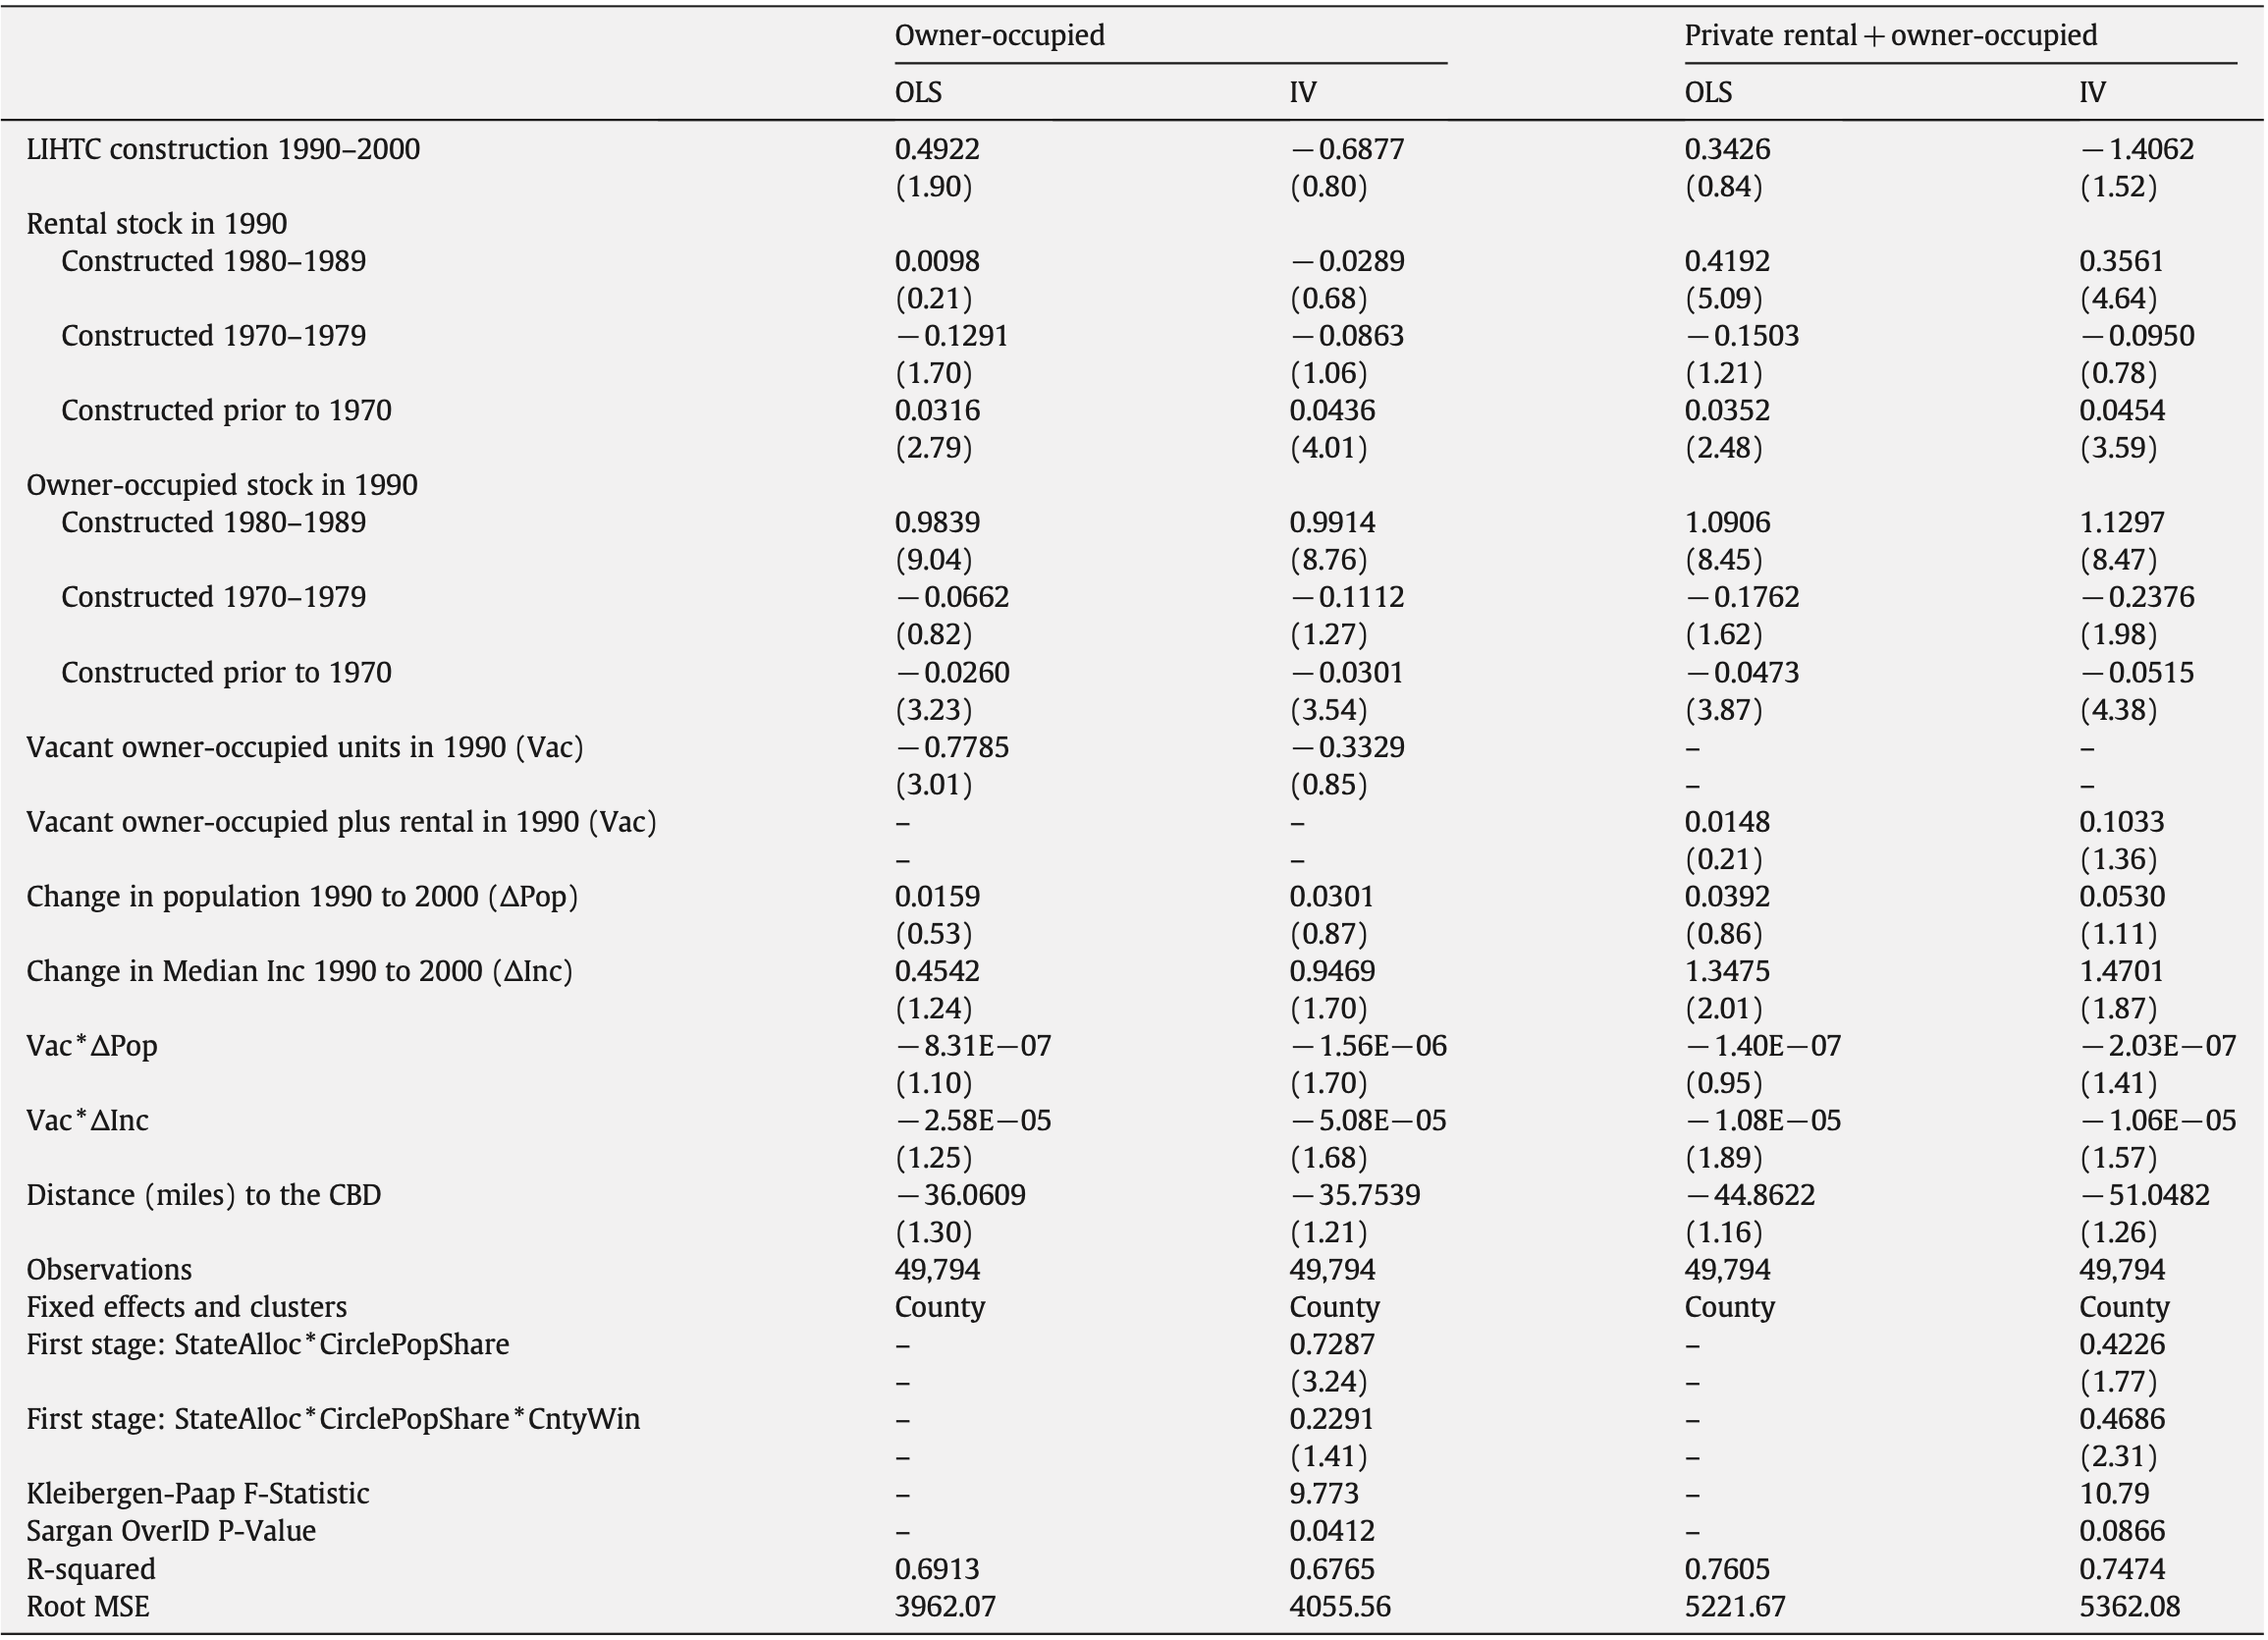
\includegraphics[width=17cm]{taba-2.png}
\end{table}

\bibliography{ref}

\end{document}
